%% 
%% Skript Differentialgeometrie im Wintersemester 12/13
%% Zur Vorlesung von Dr. Grensing am KIT Karlsruhe
%% 
%% Kapitel 9
%% 
\chapter{Jacobifelder}

F"ur $p,q \in M$ sei $\Omega_{pq}$ der Raum aller glatten Kurven
$c:[0,1] \to M$ mit $c(0)=p$ und $c(1)=q$.
\begin{center}\begin{tikzpicture}[font=\scriptsize]
    %	\tikzgitter{(-5,-5)}{(5,5)} % Hilfsgitter

    \coordinate (p) at (-3.5,-1); \coordinate (q) at ($-1*(p)$); \fill
    (p) circle(0.05)node[left]{$p$} (q) circle(0.05)node[right]{$q$}
    (0,0) circle(0.05)node[below right]{$c$};

    \coordinate (ctrl) at (2,-0.25); \draw (p) ..controls(p) and
    ($-1*(ctrl)$).. (0,0) ..controls(ctrl) and (q).. (q);

    \coordinate (a) at (0,-1); \coordinate (b) at ($-1*(a)$);
    \coordinate (ctrl2) at (0.25,0.5); \draw (a) ..controls(a) and
    ($-1*(ctrl2)$).. (0,0) ..controls(ctrl2) and (b).. (b); \draw[->]
    (0,0) -- ($2*(ctrl2)$) node[right]{$\difffrac{}{s}c_s$};

    \def\faktor{0.2} \foreach \y in {1, 2}{ \path (a) ..controls(a)
      and ($-1*(ctrl2)$).. (0,0) ..controls(ctrl2) and
      (b).. coordinate[pos=\y * \faktor] (coord) (b);
      % \draw[red] (coord) circle(0.05);
      \draw[dashed] (p) ..controls(p) and ($(coord)
      -1*(ctrl)$).. (coord) ..controls($(coord) + (ctrl)$) and
      (q).. (q); } \foreach \y in {1, 2, 3}{ \path (a) ..controls(a)
      and ($-1*(ctrl2)$).. coordinate[pos=1 - \y * \faktor] (coord)
      (0,0) ..controls(ctrl2) and (b).. (b);
      % \draw[red] (coord) circle(0.05);
      \draw[dashed] (p) ..controls(p) and ($(coord)
      -1*(ctrl)$).. (coord) ..controls($(coord) + (ctrl)$) and
      (q).. (q); }
  \end{tikzpicture}\end{center}

\begin{Dfn}
  Eine \CmMark[Variation]{(glatte) Variation} einer glatten Kurve
  $c:[a,b] \to M$ ist eine glatte Abbildung
  \begin{align*}
    h:(-\epsilon, \epsilon) \X [a,b] \to M && h_s(t) = h(s,t)
  \end{align*}
  mit $h_0 = c$. Gilt $h(\cdot, a) \equiv c(a)$ und $h(\cdot, b)
  \equiv c(b)$, so hei"st $h$ eine \CmMark[Variation!mit festen
  Endpunkten]{Variation mit festen Endpunkten} oder
  \CmMark[Variation!eigentliche]{eigentliche Variation}. Man schreibt
  $c_s$ f"ur eine Variation $h$ von $c$.
\end{Dfn}

Ist $c_s$ eine glatte Variation von $c$, so ist
\begin{align*}
  Y(t) &= \difffrac[s=0]{}{s} c_s(t)\\
  &= \difffrac[s=0]{}{s} h(s,t) =
  h_{*(0,t)}\left(\pdifffrac{}{s}\right)
\end{align*}
ein Vektorfeld entlang $c$. ist $c_s$ eigentlich, so gilt $Y(a) = 0
\in \T_{c(a)}M$ und $Y(b) = 0 \in \T_{c(b)}M$.
\begin{center}\begin{tikzpicture}[font=\scriptsize]
    \coordinate (1) at (-2,-1); \coordinate (2) at (0,0); \coordinate
    (3) at (2,1.5); \coordinate (ctrl) at (1.5,0.25); \draw (1)
    ..controls(1) and ($-1*(ctrl)$)..node[pos=0.6,below]{$c$}
    coordinate[pos=0.9] (a) (2) ..controls(ctrl) and (3)..  (3); \fill
    (a) circle(0.05); \draw[->] (a) -- ($(a) + (0.5,1)$)
    node[left]{$Y(t)$};
  \end{tikzpicture}\end{center}
Tats"achlich ist jedes Vektorfeld ein solches Variationsfeld einer
Variation von $c$: Ist $Y$ ein Vektorfeld entlang $c$, so definiert
$h(s,t) = \exp_{c(t)}(s Y(t))$ eine Variation von $c$ und es gilt:
\begin{align*}
  \difffrac[s=0]{}{s} h(s,t) &= \exp_{c(t)*0}(Y(t))\\
  &= \id_{\T_{c(t)}M}(Y(t)) = Y(t).
\end{align*}
Falls $Y$ in den Endpunkten von $c$ verschwindet, so ist die so
definierte Variation eigentlich. Bestimme $\difffrac[s=0]{}{s} E(c_s)$
und $\difffrac[s=0]{}{s}\calL(c_s)$:
\begin{align*}
  \frac{1}{2} \difffrac[s=0]{}{s} \langle \dot c_s, \dot c_s \rangle &= \langle \nabla_s \dot c(s), \dot c(s) \rangle\\
  &= \left\langle \nabla_s \difffrac{}{t} c_s, \dot c(s) \right\rangle = \left\langle \nabla_t \difffrac{}{s} c_s, \dot c_s \right\rangle \\
  &= \left\langle \difffrac[s=0]{}{s} c_s, \dot c_s \right\rangle' - \left\langle \difffrac[s=0]{}{s} c_s, \nabla_t \dot c_s \right\rangle \\
  &= \left\langle Y, \dot c \right\rangle' - \left\langle Y, \nabla_t \dot c \right\rangle\\
\end{align*}
\begin{align*}
  \difffrac[s=0]{}{t} \|\dot c_s\| &= \frac{1}{2 \|c_s\|} \difffrac[s=0]{}{s} \langle \dot c_s, \dot c_s \rangle\\
  &= \frac{\langle Y, \dot c \rangle' - \langle Y, \nabla_t \dot c
    \rangle}{\|\dot c\|}
\end{align*}
Damit folgt:
\begin{align*}
  \difffrac[s=0]{}{s} E(c_s) = \difffrac[s=0]{}{s} \int_a^b
  \frac{1}{2} \|\dot c_s\| = \left. \langle Y, \dot c \rangle
  \right|_a^b - \int_a^b \langle Y, \nabla_t \dot c \rangle
\end{align*}
Betrachte $E: \Omega_{pq} \to \R$. Dann ist $c \in \Omega_{pq}$ genau
dann eine Geod"atische, wenn $c$ ein kritischer Punkt von $E$ ist, das
hei"st $\difffrac[s=0]{}{s}E(c_s) = 0$ f"ur jede eigentliche Veriation
von $c$.  Ist $c$ ein kritischer Punkt von $E$, so sei $c_s$ die von
$Y = f \nabla_t \dot c$ mit $f(0) = 0 = f(1)$ erzeugte Variation.
Dann ist $c_s$ eigentlich und es gilt
\begin{align*}
  0 = \difffrac[s=0]{}{s} E(c_s) = - \int_a^b f \|\nabla_t \dot c\|^2
\end{align*}
also $\nabla_t \dot c = 0$.  Ist $c$ nach der Bogenl"ange
parametrisiert, so gilt
\begin{align*}
  \difffrac[s=0]{}{s} \calL(c_s) = \difffrac[s=0]{}{s} E(c_s)
\end{align*}
%% 
%% Vorlesung <2013-1-11 Fri>
%% 
Eine kurve $c \in \Omega_{pq}$ ist genau dann ein kritischer Punkt von
$\calL$, wenn $c$ eine umparametrisierte Geod"atische ist.

\section{Ausblick: Hesse \& Morse - Theorie}

Sei $f \in C^\infty(M)$, sei nach Konvention $\nabla_X f = X(f) = \dop
f(X)$, und $\nabla f = \dop f \in \Omega^1(M) = \Gamma(\T M^*)$. F"ur
die Hessesche $\Hh_f = \nabla^2 f$ gilt nach Proposition
\ref{prop-7-3}:
\begin{align*}
  \nabla^2 f (X,Y) &= (\nabla_X \dop f)(Y) = X(\dop f(Y)) - \dop f(\nabla_X Y)\\
  &= X(Yf) - (\nabla_X Y)(f) \qquad (= \nabla_{X,Y}^2 \text{ in Kapitel 7})\\
  &= [X,Y]f + Y(Xf) - (\underbrace{\nabla_X Y - \nabla_Y X}_{\mathclap{[X,Y] \text{ Torsionsfreiheit}}}) f - (\nabla_Y X) f\\
  &= Y(Xf) - (\nabla_YX)(f) = \nabla^2 f(Y,X) = \Hh_f(Y,X)
\end{align*}
Die Hessesche ist also eine symmetrische $\R$-Bilinearform $\Hh_f:
\calV(M) \X \calV(M) \to C^\infty(M)$. Sie ist im Allgemeinen
\emph{nicht} $\C^\infty(M)$-bilinear. Ist $p \in M$ ein kritischer
Punkt von $f$, das hei"st $\dop f|_p = 0$, dann h"angt $\Hh_f|_p$ nur
von $\xi = X_p$ und $\eta = Y_p$ ab: Ist $\tilde X$ ein Vektorfeld mit
$\tilde X_p = \xi = X_p$, so gilt:
\begin{align*}
  \Hh_f|_p(\tilde X,Y) &= \tilde X_p(Yf) - \underbrace{\dop f|_p(\nabla_{\tilde X}Y)}_{=0} = \tilde X_p(Yf) = \xi(Yf)\\
  &= X_p(Yf) = \ldots = \Hh_f|_p(X,Y)
\end{align*}
$\Hh_f|_p$ ist eine Bilinearform auf $\T_pM$. Insbesondere h"angt
$\Hh_f|_p$ nur von der differenzierbaren Struktur von $M$ und
\emph{nicht} von der Riemannschen Struktur ab.  Ist $\Hh_f$ nicht
ausgeartet, so hei"st die Anzahl der negativen Eigenwerte der
\CmMark{Index} von $f$ in $p$.  Ist $v \in \T_pM$ der Eigenvektor zu
einem negativen Eigenwert $k$ und $\gamma$ eine Kurve mit
$\gamma(0)=p$ und $\dot\gamma(0)=v$. Dann gilt
\begin{align*}
  0 > \lambda || v ||^2 = \Hh_f|_p (v,v) = v((f \circ \gamma)') =
  \difffrac[t=0]{^2}{t^2} f(\gamma(t))
\end{align*}
Entlang der Kurve $\gamma$ nimmt $f$ also ein striktes Maximum an.
\begin{center}\begin{tikzpicture}[font=\scriptsize,normal/.style={above,sloped,
      inner sep=0pt,outer sep=0pt,allow upside down,below}]
    % \tikzgitter{(-7,-7)}{(7,7)}
    
    % neuer Befehl f"ur die kleine Parabel (1. Parameter Scheite,
    % 2. Parameter linker Linenstil, 3. Parameter rechter Linienstil,
    % optionaler Parameter Rotation)
    \newcommand\tikzKleineParabel[4][0]{ \def\kbreite{1}
      \def\khoehe{2} \def\kstretch{0.75} \coordinate[rotate
      around={#1:#2}] (links) at ($#2 + (-\kbreite,-\khoehe)$);
      \coordinate[rotate around={#1:#2}] (rechts) at ($#2 +
      (\kbreite,-\khoehe)$);
      
      \draw[#3,rotate around={#1:#2}] (links) ..controls (links) and
      ($#2 - (\kstretch,0)$).. #2; \draw[#4,rotate around={#1:#2}] #2
      ..controls($#2 + (\kstretch,0)$) and (rechts).. (rechts); }
    
    % grosse Parabel mit den kleinen Parabeln drauf
    \def\stretch{2.5} \def\gbreite{4} \def\ghoehe{4} \coordinate
    (lende) at (-\gbreite,\ghoehe); \coordinate (rende) at
    (\gbreite,\ghoehe); \coordinate (scheitel) at (0,0); \draw (lende)
    ..controls(lende) and ($(scheitel) - (\stretch,0)$)..
    node[pos=0.4,normal]{\tikz \tikzKleineParabel{(0,0)}{dashed}{};}
    node[pos=0.7,normal]{\tikz \tikzKleineParabel{(0,0)}{dashed}{};}
    (scheitel) ..controls($(scheitel) + (\stretch,0)$) and (rende)..
    node[pos=0.3,normal]{\tikz \tikzKleineParabel{(0,0)}{}{dashed};}
    node[pos=0.6,normal]{\tikz \tikzKleineParabel{(0,0)}{}{dashed};}
    (rende);
    
    % Beschriftung
    \fill (scheitel) circle(0.05) node[above]{$p$}; \node at
    (0.5*\gbreite,0.75*\ghoehe) {$M$}; \node at
    (\gbreite,-0.5*\ghoehe) {$f$ H"ohenfunktion};
    
    % mittlere kleine Parabel und die beiden Waagrechten kleinen
    % Parabeln links und rechts
    \tikzKleineParabel{(scheitel)}{}{dashed}
    \tikzKleineParabel[270]{(lende)}{}{}
    \tikzKleineParabel[90]{(rende)}{}{}
  \end{tikzpicture}\end{center}
Tats"achlich ist jeder nicht ausgeartete kritische Punkt von solcher
Gestalt.

\begin{emptythm}[Morse-Lemma]
  Es sei $p \in M$ ein nicht ausgearteter kritischer Punkt von $f \in
  C^\infty(M)$ mit Index $\alpha$. Dann existiert eine Karte ($\phi,
  U)$ um $p$ mit $\phi(p) = 0$ und $f = f(p) - (\phi^1)^2 - (\phi^2)^2
  - \ldots -(\phi^\alpha)^2 + (\phi^{\alpha+1})^2 + \ldots +
  (\phi^m)^2$.
\end{emptythm}

\paragraph{Morse-Theorie}
\begin{center}\begin{tikzpicture}[font=\scriptsize]
    %	\tikzgitter{(-5,-5)}{(5,5)}
    
    % die grosse Ellipse
    \def\hoehe{2} \def\breite{1.25} \coordinate (mitte) at (0,0);
    \draw (mitte) ellipse({\breite} and \hoehe);
    
    % die kleinen Ellipse
    \def\kbreite{0.5} \def\khoehe{0.125} \coordinate (a) at ($(mitte)
    - (\breite,0)$); \coordinate (b) at ($(mitte) - (0.25,0)$);
    \coordinate (d) at ($(mitte) + (\breite,0)$); \coordinate (c) at
    ($(mitte) + (0.25,0)$); \coordinate (cntrl) at
    ($0.5*(a)+0.5*(b)$); \coordinate (cntrr) at ($0.5*(c)+0.5*(d)$);
    \begin{scope}
      \clip ($(mitte) - 1.1*(\breite,0)$) rectangle ($(mitte) +
      1.1*(\breite,-2*\khoehe)$); \draw (cntrl) ellipse({\kbreite} and
      {\khoehe}); \draw (cntrr) ellipse({\kbreite} and {\khoehe});
    \end{scope}
    \begin{scope}
      \clip ($(mitte) - 1.1*(\breite,0)$) rectangle ($(mitte) +
      1.1*(\breite,2*\khoehe)$); \draw[dashed] (cntrl)
      ellipse({\kbreite} and {\khoehe}); \draw[dashed] (cntrr)
      ellipse({\kbreite} and {\khoehe});
    \end{scope}
    
    % das Loch in der Mitte
    \begin{scope}
      \clip ($(mitte) + (0.5,1)$) rectangle ($(mitte) - (1, 1)$);
      \path[draw,name path=gkreis] ($(mitte) - (0.75,0)$) ellipse (1
      and 1.25);
    \end{scope}
    \path[name path=kkreis] ($(mitte) + (0.5,0)$) ellipse (0.75 and 1);
    \path[name intersections={of=gkreis and kkreis}];
    \begin{scope}
      \clip (intersection-1) rectangle ($(intersection-2)-(0.5,0)$);
      \draw ($(mitte) + (0.5,0)$) ellipse (0.75 and 1);
    \end{scope}
    
    % die Punkte
    \coordinate (p) at ($(mitte) - (0,\hoehe)$); \coordinate (q) at
    (intersection-2); \coordinate (r) at (intersection-1); \coordinate
    (s) at ($(mitte) + (0,\hoehe)$); \fill (p)
    circle(0.05)node[below]{$p=0$} (q) circle(0.05)node[below
    right]{$q$} (r) circle(0.05)node[above right]{$r$} (s)
    circle(0.05)node[above]{$s$};
    
    % der Strich
    \def\strichentfernung{2.5} \draw ($(d) +
    (\strichentfernung,-\hoehe - 0.5)$) node[below left]{$\R$} --
    ++(0,2*\hoehe+1);
    
    % der Pfeil
    \draw[->] ($(d) + 0.5*(\strichentfernung,0) - (0.5,0)$)
    --node[above]{$f$} ++(1,0);
    
    % ich bastle einen neuen Befehl f"ur die Striche mit der
    % Beschriftung
    \newcommand\beschriftung[2]{ \coordinate (pos) at ($#1 +
      (\strichentfernung+\breite,0)$); \def\weite{0.1} \draw ($(pos) -
      (\weite,0)$) -- ++(2*\weite,0) node[right,align=left]{#2}; }
    \beschriftung{(s)}{$f(s)$ Index 2\\ (glob. Max. d. H"ohenfktn.)}
    \beschriftung{(r)}{$f(r)$ Index 1}
    \beschriftung{(mitte)}{$a=f(x)$} \beschriftung{(q)}{$f(q)$ Index
      1} \beschriftung{(p)}{$f(p)=0$ Index 0}
    
    \node at ($(mitte) + (-1.75*\breite,0.75*\hoehe)$) {$M = T^2
      \subseteq \R^3$}; \node (txt) at ($(mitte) +
    (-1.75*\breite,-1*\hoehe)$) {$M^{a} = \{ f \le a \}$}; \draw[->]
    (txt) to[in=180] ($(mitte) - 0.5*(\breite,\hoehe)$);
    
  \end{tikzpicture}\end{center}
Die Topologien von $M^a$ und $M^b$ sind identisch, wenn zwischen $a$
und $b$ keine kritischen Werte auftreten.
\emph{\quot{Rekonstruktion}:} Klebe sukzessive f"ur die nicht
ausgearteten kritischen Punkte $p$ Zellen der Dimension $\Ind_f(p)$,
das hei"st $\B_1(0) \subseteq \R^{\Ind_f(p)}$.
\begin{center}\textcolor{red}{[BILD]}\end{center}
Auf jeder glatten Mannigfaltigkeit existiert einee sogenannte
\CmMark{Morse-Funktion}, das hei"st eine Funktion mit isolierten
kritschen Punkten, alle nicht entartet und $f^{-1}([a,b])$
kompakt. Ist $f(p) = a$ ein kritischer Wert, so unterscheiden sich
$M^{\alpha - \epsilon}$ und $M^{\alpha + \epsilon}$ durch das Ankleben
einer $\Ind_f(p)$-Zelle.

Weitere Informationen zu diesem Thema lassen sich im Buch \quot{Morse
  Theory} von J. Milnor \cite{milnor1963morsetheo} finden.

\section{Zweite Ableitung des Energiefunktionals (in kritischen
  Punkten)}
Es sei $c$ eine nach Bogen"ange parametrisierte Geod"atische, $c_s$
eine Variation von $c$ und $Y(t) = \difffrac[s=0]{}{s} c_s(t)$. Dann
gelten die folgenden Gleichungen:
\begin{align*}
  E(c_s) = \frac{1}{2} \int_0^{\calL} \| \dot c_s \|^2
\end{align*}
\begin{align*}
  \difffrac{}{s} \langle \dot c_s, \dot c_s \rangle &= 2 \langle \nabla_s \dot c_s, \dot c_s \rangle \\
  &= 2 \left\langle \nabla_t \difffrac{}{s} c_s, \dot c_s \right\rangle \\
  \difffrac{^2}{s^2} \langle \dot c_s, \dot c_s \rangle &= 2 \left\langle \nabla_s \nabla_t \difffrac{}{s} c_s, \dot c_s \right\rangle + 2 \left\langle \nabla_t \difffrac{}{s} c_s, \nabla_s \dot c_s \right\rangle\\
  &= 2 \left\langle \nabla_s \nabla_t \difffrac{}{s} c_s, \dot c_s
  \right\rangle + 2 \left\| \nabla_t \difffrac{}{s} c_s \right\|^2
\end{align*}
\begin{align*}
  \nabla_s \nabla_t \difffrac{}{s} c_s = \nabla_t \nabla_s
  \difffrac{}{s} c_s + R \left( \smash{\underbrace{\difffrac{}{s}
        c_s}_{\mathclap{s=0:\, Y(t)}}}, \difffrac{}{t} c_s \right)
  \difffrac{}{s} c_s \vphantom{\underbrace{\difffrac{}{a}}_{A}}
\end{align*}
Zur "Ubersichtlichkeit setzen wir nun $\nabla_t Y =: Y'$
\begin{align*}
  \frac{1}{2} \difffrac[s=0]{^2}{s^2} \langle \dot c_s, \dot c_s \rangle &= \left\langle \nabla_t \nabla_s \difffrac{}{s} c_s, \dot c_s \right\rangle + \left\langle R(Y,\dot c)Y, \dot c \right\rangle + \| \nabla_t Y \|^2\\
  &= \left\langle \nabla_s \difffrac{}{s} c_s, \dot c \right\rangle' -
  \left\langle R(Y, \dot c) \dot c, Y \right\rangle + \| Y' \|^2
\end{align*}
\begin{align*}
  \difffrac{^2}{s^2} E(c_s) = \left. \left\langle \nabla_s
      \difffrac{}{s} c_s, \dot c_s \right\rangle \right|_{0}^{\calL} +
  \int_0^{\calL} \| Y' \|^2 - \left\langle R(Y, \dot c) \dot c, Y
  \right\rangle
\end{align*}
\begin{align*}
  \difffrac[s=0]{^2}{s^2} \| \dot c_s \| &= \difffrac[s=0]{}{s} \left( \frac{1}{2 \| \dot c_s \|} \difffrac{}{s} \| \dot c \|^2 \right) \\
  &= - \frac{1}{4} \left( \difffrac[s=0]{}{s} \| c_s \|^2 \right)^2 +
  \frac{1}{2} \difffrac[s=0]{^2}{s^2} \| \dot c_s \|^2
\end{align*}
\begin{align*}
  \difffrac[s=0]{^2}{s^2} \calL(c_s) &= \difffrac[s=0]{^2}{s^2} E(c_s) - \frac{1}{4} \int \left( \difffrac[s=0]{}{s} \| \dot c_s \|^2 \right)^2 \\
  &= \left.\left\langle \nabla_s \difffrac{}{s} c_s, \dot c_s
    \right\rangle\right|_{0}^{\calL} + \int_0^{\calL} \| Y' \|^2 -
  \langle R(Y, \dot c) \dot c, Y \rangle - ( \langle Y', \dot c
  \rangle )^2
\end{align*}
Bezeichnet $Y^\perp = Y - \langle \dot c, Y \rangle \dot c$ den
Normalenanteil von $Y$ bez"uglich $\dot c$, so gilt:
\begin{align*}
  {Y^\perp}' &= Y' - \langle \nabla_t \dot c, Y \rangle \dot c - \langle \dot c, Y' \rangle \dot c - \langle \dot c, Y \rangle \nabla_t \dot c \\
  &= Y' - \langle \dot c, Y' \rangle \dot c = (Y')^\perp
\end{align*}
\begin{align*}
  \| {Y'}^\perp \| - \langle R(Y^\perp, \dot c) \dot c, Y^\perp \rangle ={}& \langle Y' - \langle \dot c, Y' \rangle \dot c, Y' - \langle \dot c, Y' \rangle \dot c \rangle - \langle R(Y, \dot c) \dot c, Y \rangle \\
  & + \langle R(Y, \dot C) \dot c, \langle \dot c, Y \rangle \dot c \rangle \\
  & + \langle R ( \langle \dot c, Y \rangle \dot c, \dot c) \dot c, Y - \langle \dot c, Y' \rangle \dot c \rangle \\
  ={}& \| Y' \|^2 - \langle R(Y, \dot c) \dot c, Y \rangle - ( \langle
  Y', \dot c \rangle )^2
\end{align*}
Es gilt:
\begin{align*}
  \difffrac[s=0]{^2}{s^2} \calL(c_s) = \left.\left\langle \nabla_s
      \difffrac{}{s} c_s, \dot c \right\rangle\right|_{0}^{\calL} +
  \int_0^{\calL} \| {Y'}^\perp \|^2 - \langle R(Y^\perp, \dot c) \dot
  c, Y^\perp \rangle
\end{align*}

%% 
%% Vorlesung <2013-1-15 Tue>
%% 

\begin{emptythm}[Erinnerung]
  Für eine glatte Funktion $f$ auf $M$ gilt in kritischen Punkten $p$:
  \begin{align*}
    H_f(v,v) = \difffrac[t=0]{^2}{t^2}f(\gamma(t))
  \end{align*}
  mit $\gamma(0) = p, \dot\gamma(0) = v$.
  Diese Eigenschaft verwenden wir in der folgenden Definition als Ausgangspunkt.
\end{emptythm}

\begin{Dfn}
  Es sei $Y$ ein Vektorfeld entlang einer nach Bogenlänge parametrisierte geod"atische Kurve $c$ und $c_s$ die von $Y$ erzeugte Variation. Die durch
  \begin{align*}
    \calI(Y,Y) = \difffrac[s=0]{^2}{s^2} E(c_s)
  \end{align*}
  auf dem Vektorraum der Vektorfelder entlang $c$ definierte symmetrische Bilinearform hei"st die \CmMark{Indexform} von $c$.
\end{Dfn}

Sind $X,Y$ Vektorfelder entlang $c$, welche in den Endpunkten
verschwinden, so gilt
\begin{align*}
  \calI(X,Y) = -\int_0^{\mathcal L}\left<X'' + R(X,\dot c)\dot
    c,Y\right>
\end{align*}
denn bezeichnet $c_s$ die von $Y$ erzeugte eigentliche Variation, so
gilt
\begin{align*}
  \difffrac[s=0]{^2}{s^2}E(c_s) & = \left.\left<\nabla_s\difffrac{}{s}c_s,\dot c\right>\right|_0^{\mathcal L} + \int_0^{\mathcal L}\|Y'\|^2 - \left<R(Y,\dot c)\dot c,Y\right>\\
  & = \int_0^{\mathcal L}\left<Y',Y\right>' - \left<Y'',Y\right> - \left<R(Y,\dot c)\dot c,Y\right>\\
  & = \left.\left<Y',Y\right>\right|_0^{\mathcal L} - \int_0^{\mathcal L} \left<Y'',Y\right> + \left<R(Y,\dot c)\dot c,Y\right>\\
  & = - \int_0^{\mathcal L}\left<Y'' + R(Y,\dot c) \dot c, Y\right>.
\end{align*}

Die Indexform um eine Geodätische $c$ ist genau dann ausgeartet, wenn ein in den Endpunkten verschwindendes Vektorfeld entlang $c$ existiert mit
\begin{align*}
  Y'' + R(Y,\dot c) \dot c \equiv 0. \tag{*}
\end{align*}

% Definition 9.3
\begin{Dfn}
  Ein Vektorfeld entlang einer Geodätischen $c$ heißt \CmMark{Jacobifeld}, wenn es die obige Differentialgleichung (*) erfüllt.
\end{Dfn}

% Lemma 9.4
\begin{Lemma}\label{thm:lemma-9-4}
  Es sei $c \colon [0,1] \to M$ eine Geod"atische, $p = c(0)$.
  Dann existiert für alle $v,w \in \T_pM$ genau ein Jacobifeld $J$ entlang $c$ mit $J(0) = v, \ J'(0) = w$.
\end{Lemma}

\begin{bew}
  Es sei $e_1, \ldots, e_m \in \T_pM$ eine Orthonormalbasis des
  Tangentialraums in $p$ und es bezeichne n $E_1, \ldots, E_m$ die
  entlang $c$ parallelen Vektorfelder mit $E_i(0) = e_i$. Dann ist
  jedes Vektorfeld $Y$ entlang $c$ von der Form $Y = \sum_i
  \eta^iE_i$. Dann gilt:
  \begin{align*}
    Y' = \sum_i (\dot \eta^i E_i + \eta^i\nabla_tE_i) = \sum_i \dot
    \eta^i E_i
  \end{align*}
  und $Y'' = \sum \ddot \eta^i E_i$. Setzt man $R(E_j,\dot c)\dot c =
  \sum_i\rho_j^i E_i$, so ist (*) äquivalent
  zum System linearer Differentialgleichungen zweiter Ordnung
  \begin{align*}
    \ddot \eta^i + \sum_i \eta^i\rho_j^i = 0.
  \end{align*}
  Existens und Eindeutigkeit folgen mit der Lösungstheorie
  gewöhnlicher Differentialgleichungen.
\end{bew}

\begin{bsp}[Jacobifelder des $\R^n$]
  Die Geodätischen des $\R^n$ sind genau die Geraden.
  Ein Vektorfeld $Y$ entlang einer Geraden ist genau dann ein Jacobifeld, wenn $Y'' = 0$ gilt; jedes solche ist der Form $Y(t) = v + tw$.
  \begin{center}\begin{tikzpicture}
      %	\tikzgitter{(-5,-5)}{(5,5)}
      
      \coordinate (0) at (0,0); \fill (0) circle(0.05);
      \def\baseangle{20}
      \def\betweenangle{20}
      \def\claenge{5}
      \def\pfeillaenge{1.5}
      \def\strichlaenge{4.5}
      
      \draw (0) --node[below right,pos=0.85]{$c$} ++(\baseangle:\claenge);
      \draw[->] (0) --node[above left]{$w$} ++(\baseangle+\betweenangle:\pfeillaenge);
      \draw[dashed] ($(0)+(\baseangle+\betweenangle:\pfeillaenge)$) -- ++(\baseangle+\betweenangle:\strichlaenge-\pfeillaenge);
      
      \def\schritt{0.125}
      \foreach \i in {0.125,0.25,...,0.75}{
        \path (0) --coordinate[pos=\i] (pkt) ++(\baseangle:\claenge);
        \path[name path=w] (0) -- ++(\baseangle+\betweenangle:1*\strichlaenge);
        \path[name path=vec] (pkt) -- ++(\baseangle+90:3);
        \path[name intersections={of=w and vec}];
        \draw[->] (pkt) -- (intersection-1);
      }
    \end{tikzpicture}\end{center}
\end{bsp}

Sind die Startwerte eines Jacobifeldes tangential an $c$, etwa $J(0) =
\lambda \dot c(0)$ und $J'(0) = \mu \dot c(0)$, so gilt
\begin{align*}
  J(t) = (\lambda + t\mu)\dot c(t),
\end{align*}
denn
\begin{align*}
  J''(t) = \nabla_t(\mu \dot c(t) + (\lambda + t \mu)\underbrace{\nabla_t\dot c(t)}_{=0}) = \mu\nabla_t\dot c = 0,\\
  \left.R(J,\dot c)\dot c\right|_t = (\lambda + t\mu)R(\dot c, \dot c)\dot c = 0.
\end{align*}
Zu $c$ tangentiale Jacobifelder tragen keine geometrischen Informationen; vgl. zweite Ableitung des Längenfunktionals.
Gilt für die Startwerte eines Jacobifeldes $J(0)$ und $J'(0) = \dot c(0)^{\perp}$
\begin{align*}
  \left<J',\dot c\right>' = \left<J'',\dot c\right> + \left<J', \nabla_t\dot c\right> = - \left<R(J,\dot c)\dot c,\dot c\right> = 0,
\end{align*}
also $J'(t) \perp \dot c(t)$ für alle Zeiten $t$ und $\left<J,\dot c\right>' = \left<J',\dot c\right> = 0$, somit $J(t) \perp \dot c(t)$ für alle $t$.

Der $\R$-Vektorraum der Jacobifelder entlang einer Geodätischen $c$ hat die Dimension $2 \dim(M)$ und die zu $c$ normalen Jacobifelder bilden einen Vektorraum der Dimension $2 \dim(M) - 2$.

% Satz 9.5
\begin{Satz}\label{satz-9-5}
  Es sei $c \colon [0,1] \to M$ eine Geodätische und $c_s$ eine Variation von $c$, so dass alle Kurven $c_s$ Geodätische sind.
  Dann ist das zugehörige Variationsfeld ein Jacobifeld entlang $c$.
  Jedes Jacobifeld ist von dieser Gestalt.
\end{Satz}

\begin{bew}
  Es sei $c_s$ eine Variation von $c$ und alle $c_s$ seien
  Geodätische. Dann gilt:
  \begin{align*}
    Y'' & = \left.\nabla_t \left(\nabla_t\difffrac{}{s}c_s \right)\right|_{s=0} \\
    & = \left.\nabla_t \left(\nabla_s\difffrac{}{t}c_s \right)\right|_{s=0}\\
    & = \nabla_s\underbrace{\nabla_t \difffrac{}{t} c_s}_{=0} + \left. R\left(\smash{\underbrace{\difffrac{}{t}c_s}_{=\dot c},\underbrace{\difffrac{}{s}c_s}_{=Y}}\vphantom{\difffrac{}{}}\right) \smash{\underbrace{\difffrac{}{t}c_s}_{=\dot c}}\right|_{s=0}\\
    & = -R(Y,\dot c)\dot c
  \end{align*}
  Es sei umgekehrt $J$ ein Jacobifeld entlang $c$, $\gamma$ die durch
  $\gamma(0) = c(0), \ \dot \gamma(0) = J(0)$ definierte Geodätische,
  sowie $V$ und $W$ die entlang $\gamma$ parallelen Vektorfelder mit
  $V(0) = \dot c(0)$ und $W(0) = J'(0)$. Dann ist
  \begin{align*}
    c_s(t) = \exp_{\gamma(s)}(t(V(s) + sW(s)))
  \end{align*}
  eine Variation von $c$ und alle Kurven $c_s$ sind Geodätische.
  Das zugehörige Variationsfeld $Y = \difffrac[s=0]{}{s} c_s$ ist nach
  dem oben Bewiesenen ein Jacobifeld. Es gilt
  \begin{align*}
    Y(0) = \difffrac[s=0]{}{s}\exp_{\gamma(s)}(0) =
    \difffrac[s=0]{}{s}\gamma(s) = J(0).
  \end{align*}
  und 
  \begin{align*}
    Y'(0) & = \left.\nabla_t\difffrac[s=0]{}{s}c_s\right|_{t=0}\\
    & = \nabla_s\difffrac[t=0]{}{t}\left.\exp_{\gamma(s)}(t(V(s) +
      sW(s)))\right|_{s=0}\\
    & = \left.\nabla_s(V(s) + sW(s))\right|_{s=0}\\
    & = V'(0) + W(0) + 0W'(0)\\
    & = W(0) = J'(0)
  \end{align*}
  Nach Lemma \ref{thm:lemma-9-4} stimmen $J$ und $Y$ überein.
\end{bew}

\begin{emptythm}[Erinnerung (Korollar \ref{thm:kor-8-12} \ref{thm:kor-8-12-iii})]
  Die zusammengesetzte Kurve oben ist k"urzer als die durchgezogene Kurve unten.
  \begin{center}\begin{tikzpicture}[font=\scriptsize,scale=0.8]
      % \tikzgitter{(-5,-5)}{(5,5)}
      
      \coordinate (p) at (-3,-2); \coordinate (ende) at (3,3);
      \coordinate (ctrlp1) at (2,0.25); \coordinate (ctrlende) at (-0.5,-3); \coordinate (ctrlende) at (-0.5,-2.75);
      \fill (p) circle(0.05)node[below]{$p$};
      
      % Zeichen die Kurve und definiere den Punkt q auf der Kurve
      \draw (p) ..controls($(p) + (ctrlp1)$) and ($(ende) + (ctrlende)$)..node[below right]{$c$} coordinate[pos=0.8] (q) coordinate[pos=0.95] (d) (ende);
      \fill (q) circle(0.05)node[below right]{$q$};
      
      \coordinate (ctrlp2) at (1,2.5); \coordinate (ctrlq) at (-1.5,0);
      \draw (p) ..controls($(p) + (ctrlp2)$) and ($(q) + (ctrlq)$)..node[above left]{$\overline c$} coordinate[pos=0.75] (e) (q);
      
      \fill (d) circle(0.05) (e) circle(0.05);
      
      \draw (e) ..controls(2,1.5) and (2.5,2).. (d);
    \end{tikzpicture}\end{center}
\end{emptythm}

% Definition 9.6
\begin{Dfn}
  Ein Punkt $p \in M$ heißt zu $q$ \CmMark{konjugiert}, wenn $q$ ein singulärer Wert von $\exp_p$ ist.
  $p$ heißt \CmMark[konjugiert!entlang einer Geodätischen]{konjugiert zu $\bm{q}$ entlang der Geodätischen $\bm{c}$}, wenn $\exp_{p*\dot c(0)}$ singulär ist, das hei"st $\Kern \exp_{p*\dot c(0)} \neq \{0\}$.
\end{Dfn}

% Proposition 9.7
\begin{Prop}
  Ein Punkt $p$ ist gnau dann konjugiert zu $q$ entlang einer
  Geodätischen $c$, wenn es ein nichttriviales Jacobifeld entlang $c$
  gibt, welches in den Endpunkten verschwindet.
\end{Prop}

\begin{center}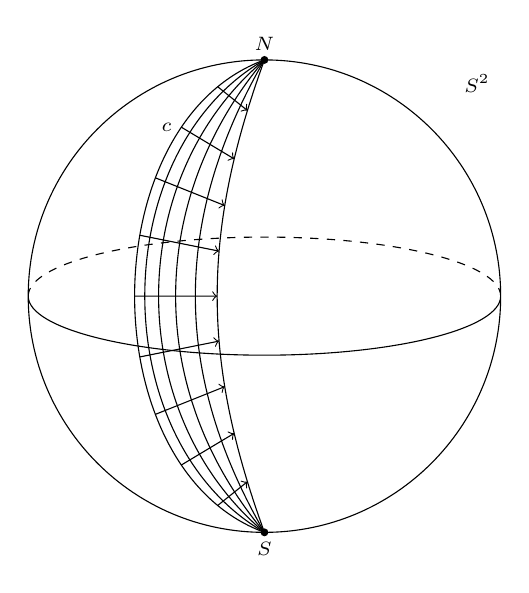
\begin{tikzpicture}[font=\scriptsize]
    % Kreis
    \def\radius{3}
    \draw (0,0) circle (\radius);
    % Ellipse
    \def\kleinradius{0.75}
    \begin{scope}
      \clip (-\radius,0) rectangle (\radius,1);
      \draw[dashed] (0,0) ellipse[x radius=\radius,y radius=\kleinradius];
    \end{scope}
    \begin{scope}
      \clip (-\radius,0) rectangle (\radius,-1);
      \draw (0,0) ellipse[x radius=\radius,y radius=\kleinradius];
    \end{scope}
    % Beschriftungen
    \coordinate (N) at (0,\radius); \coordinate (S) at (0,-\radius);
    \fill (N) circle (0.05) node[above]{$N$} (S) circle (0.05) node[below]{$S$};
    \node at (0.9*\radius,0.9*\radius) {$S^2$};
    % Boegen
    \def\firstangle{20}
    \draw (N) to[out=180+\firstangle,in=180-\firstangle] node[left,pos=0.2]{$c$} (S);
    \def\stepangle{10}
    \foreach \i in {1,2,...,5}{
      \draw (N) to[out=180 + \firstangle + \i * \stepangle,in=180-\firstangle - \i * \stepangle] (S);
    }
    \foreach \i in {0.1,0.2,...,0.9}{
      \path (N) to[out=180+\firstangle,in=180-\firstangle] coordinate[pos=\i] (a) (S);
      \path (N) to[out=180 + \firstangle + 5 * \stepangle,in=180-\firstangle - 5 * \stepangle] coordinate[pos=\i] (b) (S);
      \draw[->] (a) -- (b);
    }
  \end{tikzpicture}\end{center}


%% 
%% Vorlesung <2013-1-18 Fri>
%% 

\begin{bew}
  Nach Satz \ref{satz-9-5} ist jedes Jacobifeld $\calJ$ entlang $c$ mit $\calJ(0) = 0$ von der Gestalt $\calJ(t) = \difffrac[s=0]{}{s} \exp_p(t(\dot c(0) + s\calJ'(0))$, oder allgemein $\difffrac[s=0]{}{s} \exp_{\gamma(s)} (t(V(s) + sW(s)))$.
  Es gilt dann
  \begin{align*}
    \calJ(1) = \difffrac[s=0]{}{s} \exp_p (\dot c(0) + s \calJ'(0)) = \exp_{p*\dot{c}(0)} (\calJ'(0))
  \end{align*}
  Damit existiert genau dann ein nichttriviales Jacobifeld $\calJ$ entlang $c$ mit $\calJ(0) = 0$, $\calJ(1) = 0$, wenn $\Kern \exp_{p*\dot{c}(0)} \ne \{0\}$.
\end{bew}

\begin{bem}\begin{enumerate}[label=\arabic*),leftmargin=*]
  \item
    Der Raum der nichttrivialen Jacobifelder mit verschwindenden Endpunkten entlang $c$ hat genau die Dimension $\ddim \Kern \exp_{p*\dot{c}(0)}$.
  \item
    Ist $p$ konjugiert zu $q$, so ist $q$ konjugiert zu $p$.
  \item
    F"ur jedes Jacobifeld $\calJ$ entlang $c$ mit $\calJ(0) = 0 = \calJ(1)$ gilt $\langle \calJ, \dot c \rangle = \langle \calJ', \dot c \rangle = 0$, denn
    \begin{align*}
      \langle \calJ', \dot c \rangle' = \langle \calJ'', \dot c \rangle = - \langle R(\calJ, \dot c) \dot c, \dot c \rangle = 0,
    \end{align*}
    also ist $\langle \calJ', \dot c \rangle = \langle \calJ, \dot c \rangle'$ konstant. Ferner gilt $\langle \calJ(0), \dot c (0) \rangle = 0 = \langle \calJ(1), \dot c(1) \rangle$, also ist $\langle \calJ, \dot c \rangle \equiv 0$.
  \item
    Sind $p$ und $q$ nicht entlang $c$ zueinander konjugiert, dann ist jedes Jacobifeld $\calJ$ entlang $c$ eindeutig durch $\calJ(0)$ und $\calJ(1)$ bestimmt, denn sind $\calJ$ und $\tilde\calJ$ Jacobifelder mit identischen Randwerten, so ist $\calJ - \tilde\calJ$ ein Jacobifeld welches in den Endpunkten verschwindet.
  \item
    Zwei Punkte sind genau dann konjugiert entlang der Geod"atischen $c$, wenn eine eigentliche geod"atische Variation von $c$ existiert.
  \end{enumerate}\end{bem}

\begin{Satz}\label{satz-9-8}
  Es seien $p, q \in M$ und sei $c: [0,1] \to M$ eine Geod"atische von $p$ nach $q$.\begin{enumerate}[label=(\roman*),widest=ii]
  \item
    Ist entlang $c$ kein Punkt zu $p$ konjugiert, dann existiert eine Umgebung $U$ von $c$ in $\Omega_{pq}$, so dass $\calL(\tilde c) > \calL(c)$ und $E(\tilde c) \ge E(c)$ f"ur alle $\tilde c \in U$ gelten.
  \item
    Falls ein $t_0 \in (0,1)$ existiert, so dass $p = c(0)$ zu $c(t_0)$ entlang $c$ konjugiert ist, so existiert eine eigentliche Variet"at $c_s$ von $c$ mit $\calL(c_s) < \calL(c)$ und $E(c_s) < E(c)$ f"ur hinreichend kleine $s$.
  \end{enumerate}\end{Satz}

\begin{Lemma}[globales Gau"s Lemma]
  Es seien $v, w \in \T_pM$ und $c(t) = \exp_p(t \cdot v)$. Dann gilt
  \begin{align*}
    \langle \exp_{p*tv}(v), \exp_{p*tv}(w) \rangle = \langle v, w \rangle.
  \end{align*}
  Insbesondere ist jede Geod"atische in $p$ orthogonal zu der Abstandssph"are
  \begin{align*}
    S_r(p) = \{ q | d(p, q) = r \}.
  \end{align*}
\end{Lemma}

\begin{bew}
  $Y$ sei das durch die Startwerte $Y(0) = 0$ und $Y'(0) = \frac{w}{t}$ bestimmte Jacobifeld entlang $c$. Dann gilt:
  \begin{align*}
    Y(t) &= \difffrac[s=0]{}{s} \exp_{\gamma(s)}(t(V(s) + sW(s))) & \gamma(0) = p, \dot\gamma(0) = Y(0) = 0\\
    &= \difffrac[s=0]{}{s} \exp_p\left(t \left(v + s \frac{w}{t}\right)\right) & V(s) = V(0) = \dot c(0) = v\\
    &= \exp_{p*tv}(w) & W(s) = \ldots = \frac{w}{t}
  \end{align*}
  Es sei $\frac{w}{t} = \lambda v + u$ mit $u \perp v$. Der zu $c$ tangentiale Anteil von $Y$ ist dann
  \begin{align*}
    Y^T(s) = \lambda s \dot c (s),
  \end{align*}
  denn ${Y^T}{''} = 0$ und $R(Y^T, \dot c) \dot c = \lambda s R(\dot c, \dot c) \dot c = 0$.
  Also gilt $Y(t) = \lambda t \dot c(t) + Y^\perp(t)$, wobei $Y^\perp$ der zu $c$ orthogonale Anteil von $Y$ ist. Es folgt
  \begin{align*}
    \langle \exp_{p*tv}(v), \exp_{p*tv}(w) \rangle &= \left\langle \difffrac{}{t} \smash{\underbrace{\exp_p(tv)}_{=c}}, Y(t) \right\rangle \vphantom{\underbrace{\difffrac{}{}}_{a}} \\
    &= \langle \dot c(t), \lambda t \dot c(t) + Y^\perp(t) \rangle \\
    &= \lambda t \|\dot c(t) \|^2 = \lambda t \|v\|^2 \\
  \end{align*}
  \begin{align*}
    \langle v, w \rangle &= \langle v, t(\lambda v + w) \rangle = t \lambda \|v\|^2
  \end{align*}
\end{bew}

% Lemma 9.10
\begin{Lemma}\label{thm:lemma-9-10}
  Es sei $c \colon [0,1] \to M$ eine Geodätische, $v = \dot c(0) \in \T_{p}M$ und $\psi$ (stückweise) glatte Kurve in $\T_pM$ mit $\psi(0) = 0$ und $\psi(1) = v$, dann gilt
  \begin{align*}
    \mathcal L(\exp_p \circ \psi) \geq \mathcal L(c),
  \end{align*}
  wobei Gleichheit genau dann gilt, wenn $\psi$ eine monotone Reparametrisierung von $t \mapsto tv$ ist.
\end{Lemma}

\begin{bew}
  Es seien $\rho$ und $\theta$ glatt, so dass $\psi = \rho \theta$ mit $\|\theta\| \equiv 1$ (Polarkoordinaten).
  \begin{align*}
    \|(\exp_p \circ \psi)'\|^2 ={}& \|\exp_{p*\rho\theta} ( \rho' \theta + \rho \theta') \|^2 \\
    ={}& {\rho'}{^2} \underbrace{\langle \exp_{p*\rho\theta} (\theta), \exp_{p*\rho\theta} (\theta) \rangle}_{= \langle \theta, \theta \rangle = 1} \\
    & + 2\rho\rho' \underbrace{\langle \exp_{p*\rho\theta} (\theta), \exp_{p*\rho\theta} (\theta') \rangle}_{= \langle \theta, \theta' \rangle = \frac{1}{2} \|\theta\|^2{'} = 0} \\
    & + \rho^2 \langle \exp_{p*\rho\theta} (\theta'), \exp_{p*\rho\theta} (\theta') \rangle \\
    ={}& {\rho'}{^2} + \rho^2 \| \exp_{p*\psi}(\theta') \|^2
  \end{align*}
  Damit folgt
  \begin{align*}
    \calL(\exp_p \circ \psi) \ge \int_0^1 | \rho' | \ge | \rho(1) - \rho(0) | = \|v\| = \calL(c)
  \end{align*}
  Gleichheit gilt genau dann, wenn $\theta$ konstant und $\rho$ monoton ist.
\end{bew}

\begin{bew}[von Satz \ref{satz-9-8}]\begin{enumerate}[label=(\roman*),leftmargin=*,widest=ii]
  \item
    Es sei $c \colon [0,1] \to M$ eine Geodätische, seien $p = c(0)$ und $q = c(1)$ und es existieren keine zu $p$ konjugierten Punkte entlang $c$.
    Es bezeichne $\phi \colon [0,1] \to \T_pM$ mit $\phi(t) = tv$. Für jedes $t \in [0,1]$ ist nach Voraussetzung $\exp_{p*\phi(t)}$ regulär, also eine lokaler Diffeomorphismus.
    Es sei $\{W_i\}$ eine endliche offene Überdeckung von $\phi([0,1])$, so dass $\exp_p|_{W_i} \colon W_i \to \exp_p(W_i) = U_i$ ein Diffeomorphismus ist.
    
    \emph{Ziel:} Lifte Variationen von $M$ nach $\T_pM$.
    \begin{center}\begin{tikzpicture}[font=\scriptsize]
        % \tikzgitter{(-5,-5)}{(5,5)}
        
        \coordinate (a) at (-2.5,-1); \coordinate (b) at (3,2.5); % Endpkte. der Kurve
        \coordinate (ctrla) at (1,2); \coordinate (ctrlb) at (-2,-0.5); % Controls Punkte fuer die Kruemmung
        \coordinate (c) at ($(a) + (ctrla)$); \coordinate (d) at ($(b) + (ctrlb)$); % die daraus entstehenden Tangentialvektoren
        
        \draw (a) ..controls(c) and (d).. coordinate[pos=0.6] (beschr) (b); % die Hauptkurve
        \draw[->] (-0.5,2.5) node[left]{$c$} to[out=340,in=110] (beschr); % die Beschriftung
        
        \def\schlauchbreite{0.25cm}
        \def\schlauchweite{0.25cm}
        % Eckpunkte fuer den Schlauch, ueber- und unterhalb der Endpkte. und daneben
        \coordinate (0) at ($(a)!\schlauchbreite!90:(c)$); \coordinate (1) at ($(b)!\schlauchbreite!270:(d)$); \coordinate (2) at ($(b)!-\schlauchweite!0:(d)$);
        \coordinate (3) at ($(b)!\schlauchbreite!90:(d)$); \coordinate (4) at ($(a)!\schlauchbreite!270:(c)$); \coordinate (5) at ($(a)!-\schlauchweite!0:(c)$);
        % diese Vektoren geben die Verschiebung gegenueber den Endpktn. an
        \coordinate (shiftavert) at ($0.5*(0) - 0.5*(a)$); \coordinate (shiftbvert) at ($0.5*(1) - 0.5*(b)$);
        \coordinate (shiftahor) at ($0.5*(5) - 0.5*(a)$); \coordinate (shiftbhor) at ($0.5*(2) - 0.5*(b)$);
        % \draw[red] (0) circle(0.05) (1) circle(0.05) (2) circle(0.05) (3) circle(0.05) (4) circle(0.05) (5) circle(0.05);
        % der Schlauch
        \draw[dashed] (0) ..controls($(0) + (ctrla)$) and ($(1) + (ctrlb)$).. (1) ..controls($(1) + (shiftbhor)$) and ($(2) + (shiftbvert)$).. (2) ..controls($(2) - (shiftbvert)$) and ($(3) + (shiftbhor)$)..
        (3) ..controls($(3) + (ctrlb)$) and ($(4) + (ctrla)$).. (4) ..controls($(4) + (shiftahor)$) and($(5) - (shiftavert)$).. (5) ..controls($(5) + (shiftavert)$) and($(0) + (shiftahor)$).. (0) -- cycle;
        
        \draw[->] (4.5,3.5) node[right]{$\epsilon$-Schlauch} to[out=180,in=45] (1);
        
        \foreach \i in {0, 0.2, ...,1}{ % Kreise entlang der Kurve
          \path (a) ..controls(c) and (d).. coordinate[pos=\i] (p) (b);
          \draw (p) circle(0.8);
        }
        \node at (1,0.75) {$U_i$};
      \end{tikzpicture}\end{center}
    Es sei $t_i$ eine Partition von $[0,1]$, so dass $\phi([t_{i-1},t_i]) \subseteq W_i$. Ist $c_s$ eine Variation von $c$, so kann $\epsilon > 0$ so gewählt werden, dass
    \begin{align*}
      c_s \colon [t_{i-1},t_i]\X(-\epsilon,\epsilon) \to U_i = \exp_p(W_i)
    \end{align*}
    gilt. Dies definiert eine Variation $\psi_s$ von $\phi$ wie folgt:
    Ist $\psi_s$ bis $t_{i-1}$ definiert und gilt $\psi_s(t_{i-1}) \in W_i$, so setzt man $\psi_s(t) = \exp_p|_{W_i}^{-1}(c_s(t))$.
    Nach Lemma \ref{thm:lemma-9-10} gilt also
    \begin{align*}
      \mathcal L(\exp_p\circ \psi_s) = \mathcal L(c_s) \geq \mathcal L(c)
    \end{align*}
    für alle $s$. Mit der Cauchy-Schwarz Ungleichung folgt dann:
    \begin{align*}
      E(c_s) \geq \frac{1}{2} \mathcal L(c_s)^2 \geq \frac{1}{2} \mathcal
      L(c)^2 = E(c)
    \end{align*}
  \item
    Es sei $c(t_0)$ entlang $c$ zu $p = c(0)$ konjugiert.
    
    \begin{description}\item[Behauptung:] Dann existiert ein zu $c$ orthogonales Vektorfeld $Y$ entlang der Geodätischen $c$ mit $Y(0) = 0$, $Y(1) = 0$ und $\calI(Y,Y) = 0$.\end{description}
    Dann gilt für die zugehärige eigentliche Variation $c_s$ von $c$:
    \begin{align*}
      \difffrac[s=0]{}{s}\mathcal L(c_s) = \lambda
      \difffrac[s=0]{}{s}E(c_s) = 0
    \end{align*}
    und, da $Y$ normal ist,
    \begin{align*}
      \difffrac[s=0]{^2}{s^2}\mathcal L(c_s) = \difffrac[s=0]{^2}{s^2}
      E(c_s) = \calI(Y,Y) < 0
    \end{align*}
    Somit ist $c$ lokales Maximum.
    \begin{description}\item[Beweis der Behauptung:]
      Es existiert ein nichttriviales (zu $c$ orthogonales) Jacobifeld $\calJ$ entlang $c|_{[0,t_0]}$ mit $\calJ(0) = 0$ und $\calJ(t_0) = 0$.
    %% 
    %% Vorlesung <2013-1-22 Tue>
    %% 
    \emph{Erinnerung:} Ist $c \in \Omega_{pq}$ eine Geodätische und $t_o \in (0,1)$, so dass $c(t_0)$ zu $p = c(0)$ entlang $c$ konjugiert ist, so existiert ein Vektorfeld $Y$ entlang $c$ mit $\calI(Y,Y) < 0$.

    \begin{center}
      \textcolor{red}{Abbildung 1: Wdh: Sphäre}
    \end{center}
	\begin{description}[font=\normalfont\itshape]
    \item[Beweis der Existenz von $Y$:] Da $c(t_0)$ zu $p$ entlang $c$ konjugiert ist, existiert ein nichttriviales Jacobifeld $J$ entlang $c|_{[0,t_0]}$ mit $J(0) = 0, J(t_0) = 0$.
    \end{description}
    Es sei $X$ das entlang $c$ parallele Vektorfeld mit $X(t_0) = -J'(t_0)$
    (nach Lemma \ref{thm:lemma-9-4} ist $J'(t_0) \neq 0)$ und
    $\alpha\colon[0,1] \to \R$ mit $\alpha(0) = 0 = \alpha(1)$ und
    $\alpha(t_0) = 1$. Für $z = \alpha \cdot X$ und $\eta > 0$ sei
    \begin{align*}
      Y(t) =
      \begin{cases}
        J(t) + \eta \cdot Z(t) & \text{ für } 0 \leq t \leq t_0\\
        \eta \cdot Z(t) & \text{ für } t_0 < t \leq 1
      \end{cases}
    \end{align*}
    $Y$ ist nun stückweise glatt, die Variantionsformeln für $\mathcal L$ und $E$, beziehungsweise die Indexform lassen sich aber ganz analog für stückweise glatte Vektorfelder beziehungsweise Variationen formalisieren.
    Es gilt, da $Y$ orthogonal zu $c$ ist, für die zu $Y$ gehörigen Variationen $c_s$:
    \begin{align*}
      J(Y,Y) = & \difffrac[s=0]{^2}{s^2}E(c_s) = \difffrac[s=0]{^2}{s^2} \mathcal L(c_s)\\
      = &{} \int_0^1\|Y'\|^2 - \left<R(Y,\dot c)\dot c,Y\right>\\
      = &{} \int_0^{t_0}\left<J',J'\right> - \left<R(J,\dot c)\dot c,J\right>\\ 
	    &+ 2 \eta\int_0^{t_0} \left< J',Z'\right> - \left< R(J,\dot c)\dot c,Z\right>\\
        & + \eta^2 \int_0^1 \left<Z',Z'\right> - \left<R(Z,\dot c)\dot c,Z\right>
    \end{align*}
    und mit 
    \begin{align*}
      \left<J',J\right>' &= \left<J',J'\right> + \left<J'',J\right> \\
      	&= \left<J',J'\right> - \left<R(J,\dot c)\dot c,J\right>\\
      \left<J',Z\right>' &= \left<J',Z'\right> + \left<J'',Z\right> \\
      	&= \left<J',Z'\right> - \left<R(J,\dot c) \dot c,Z\right>
    \end{align*}
    folgt
    \begin{align*}
      J(Y,Y) & = \left<J',J\right>|_0^{t_0} + 2 \eta \left<J',Z\right>|_0^{t_0} + \eta^2J(Z,Z)\\
      & = 0 + 2 \eta\left(\left<J'(t_0),Z(t_0) \right> - \left<J'(0),Z(0)\right>\right) + \eta^2 J(Z,Z)\\
      & = -2\eta \|J'(t_0)\|^2 + \eta^2J(Z,Z)
    \end{align*}
    Für hinreichend kleines $\eta > 0$ ist damit $\calJ(Y,Y) < 0$.
    \end{description}
  \end{enumerate}\end{bew}

Betrachte die Sphäre vom Radius $r > 0$, $S^n_r \subseteq \R^{n+1}$:

\begin{center}
\begin{tikzpicture}[font=\scriptsize]
%	\tikzgitter{(-5,-5)}{(5,5)}
	\def\radius{3}
	\def\kradius{1.25}
	
	\draw (0,0) circle(\kradius) (0,0) circle(\radius);
	\def\fraction{0.5}
	\begin{scope}
		\clip (-\radius,0) rectangle (\radius,\radius);
		\draw[dashed] (0,0) ellipse[x radius=\radius,y radius = \fraction*\radius] (0,0) ellipse[x radius=\kradius,y radius = \fraction];
	\end{scope}\begin{scope}
		\clip (-\radius,0) rectangle (\radius,-\radius);
		\draw (0,0) ellipse[x radius=\radius,y radius = \fraction*\radius] (0,0) ellipse[x radius=\kradius,y radius = \fraction];
	\end{scope}
	
	\coordinate (p) at (2.25,1.75);
	\fill (p) circle(0.05) node[above left]{$p$};
	\draw[->] (0,0) --coordinate[pos=0.4] (pkt) (p) coordinate[pos=0.9] (a) (p) --node[right]{$v$} coordinate[pos=0.1] (b) (1.5,-1.75);
	\draw[dashed,name path=a] (0,0) -- (1.5,-1.75);
	
	\draw (a) edge[bend right=30] (b);
	\fill ($(p) + 0.8*0.5*(a) + 0.8*0.5*(b) - 0.8*(p) $) circle(0.025);
	
	\coordinate (vec) at ($(1.5,-1.75) - (p)$);
	
	\path[name path=b] (pkt) -- ++(vec);
	\path[name intersections={of=a and b}];
	\draw[->] (pkt) -- (intersection-1);
	
	\node at (-1.25,1) {$S^n$}; \node at (-2,2.5) {$S_r^n$};
\end{tikzpicture}\end{center}

Als differenzierbare Mannigfaltigkeit ist $S^n_r$ diffeomorph zur Standardsphäre $S^n = S^n_1$, vermöge der Abbildung $p \mapsto \frac{1}{r}p$. Bezeichnet $\left<\cdot,\cdot\right>_r$, die von
$\R^{n+1}$ auf $S^n_r$ induzierte Riemannsche Metrik, so sind $(S^n_r,\left<\cdot,\cdot\right>_r)$ und $(S^n,r^2\left<\cdot,\cdot\right>_1)$ isometrisch.
Es folgt also $\diam(S^n_r,\left<\cdot,\cdot\right>_r) = \pi r = r \diam(S^n,\left<\cdot,\cdot\right>_1)$.
Für die Schnittkrümmung einer von $v,w \in \T_pM$ aufgespannte Ebene
\begin{align*}
  \sec_p^{S^n_r}(\{v,w\}) & =
  \frac{\left<R(v,w)w,r\right>_r}{\|v\|_r^2\|w\|_r^2-\left<v,w\right>_r}
  =
  \frac{r^2\left<R(v,w)w,v\right>_1}{r^4(\|v\|_1^2\|w\|_1^2-\left<v,w\right>_1)}\\
  & = \frac{1}{r^2} \sec_p^{S^n}(\{v,w\}) = \frac{1}{r^2}.
\end{align*}
Insbesondere gilt für die Ricci-Krümmung:
\begin{align*}
  \ric_p^{S_r^n}(v,v) & = \sum_i \left<R\left(e_i,\frac{v}{\|v\|_1}\right)\frac{v}{\|v\|_1},e_i\right>\\
  & = \|v\|_1^2\sum_{i \geq 2}\sec_p^{S^n_r}(\{v,e_i\}) = \|v\|_1^2 \frac{1}{r^2}(n-1)\\
  & = (n-1)\frac{1}{r^2}\left<v,v\right>_1.
\end{align*}
wobei $\{\frac{v}{\|v\|_1}, e_2, \ldots, e_n\}$ eine Orthonormalbasis ist.

% Satz 9.11
\begin{Satz}[Bonnet-Myers]
  Es sei $(M,g)$ eine vollständige $m$-dimensionale Riemannsche Mannigfaltigkeit mit 
  \begin{align*}
    \ric_p \geq (m-1) \frac{1}{r^2} g
  \end{align*}
  für ein $r > 0$.
  Dann gilt
  \begin{align*}
    \diam(M,g) \leq \pi r = r \diam(S^m,\left<\cdot,\cdot\right>_1).
  \end{align*}
  Insbesondere ist $M$ kompakt.
\end{Satz}

\begin{bew}
  Es sei $l < \diam(M,g)$.
  Dann existieren $p,q \in M$ mit $\d(p,q) = l$ und nach dem Satz von Hopf-Rinow eine minimale Geodätische $c\colon[0,l] \to M$ von $p$ nach $q$.
  Für jedes Vektorfeld $Y$ entlang $c$, welches in den Endpunkten verschwindet, ist $J(Y,Y) \geq 0$.
  Es sei $\dot c(0) = e_1, \ldots, e_m \in \T_pM$ eine Orthonormalbasis und $E_i$ die entlang $c$ parallelen Vektorfelder mit $E_i(0) = e_i$ für $i \leq m$.
  Für 
  \begin{align*}
    Y_i(t) & = \sin \left(\frac{\pi}{l}t \right) E_i(t)\\
    0  \leq J(Y_i,Y_i) &= -\int\limits_0^l\left<Y_i''+R(Y_i,\dot c)\dot c,Y_i\right>\\
    & = -\int\limits_0^l\left<-\frac{\pi^2}{l^2}\sin\left(\frac{\pi}{l}t\right)E_i(t) + \sin\left(\frac{\pi}{l}t\right)R(E_i,\dot c)\dot c|_t,\sin\left(\frac{\pi}{l}t\right)E_i(t)\right>\\
    & = \int\limits_0^l \sin^2\left(\frac{\pi}{l}t\right)\left(\frac{\pi^2}{l^2}-\left<R(E_i,\dot c)\dot c,E_i(t)\right>\right).
  \end{align*}
  Es folgt
  \begin{align*}
    0 \leq \sum_{i \geq 2}J(Y_i,Y_i) = \int\limits_0^l\sin^2\left(\frac{\pi}{l}t\right)\Big(\underbrace{(m-1)\frac{\pi^2}{l^2} - \ric(\dot c(t),\dot c(t))}_{\leq (m-1)\left(\frac{\pi^2}{l^2}-\frac{1}{r^2}\right)}\Big)
  \end{align*}
  und somit $\frac{\pi^2}{l^2} - \frac{1}{r^2} \geq 0$, also $l \leq \pi r$.
\end{bew}

\begin{bem}\begin{enumerate}[label=(\arabic*),leftmargin=*]
\item
	Die Existenz einer uniformen positiven Krümmungsschranke ist entprechend
	\begin{align*}
		M = \{x \in \R^3 \mid x_1^2 + x_2^2 - x_3^2 = -1, x_3 > 0\}
	\end{align*}
	\begin{center}\begin{tikzpicture}
		%\tikzgitter{(-3,-3)}{(3,3)}
		\def\hor{1.5}
		\def\vert{1}
		\draw[dashed,thin] (-\hor,-\vert) -- (\hor,\vert) (-\hor,\vert) -- (\hor,-\vert);
		
		\def\abzug{0.1}
		\draw (-\hor+\abzug,\vert) ..controls(-\hor+\abzug,\vert) and (-0.5,0.25).. coordinate[pos=0.3](a) coordinate[pos=0.6](b) (0,0.25) ..controls(0.5,0.25) and (\hor-\abzug,\vert).. coordinate[pos=0.4](c) coordinate[pos=0.7](d) (\hor-\abzug,\vert);
		%\fill[red] (a) circle(0.05) (b) circle(0.05) (c) circle(0.05) (d) circle(0.05);
		
		\begin{scope}
			\clip (a) rectangle ($(d)+(0,0.25)$);
			\draw[dashed] let \p1=($0.5*(d)-0.5*(a)$) in ($0.5*(d) + 0.5*(a)$) ellipse[x radius={veclen(\x1,\y1)},y radius=0.125cm];
		\end{scope}\begin{scope}
			\clip (b) rectangle ($(c)+(0,0.25)$);
			\draw[dashed] let \p1=($0.5*(c)-0.5*(b)$) in ($0.5*(c) + 0.5*(b)$) ellipse[x radius={veclen(\x1,\y1)},y radius=0.1cm];
		\end{scope}\begin{scope}
			\clip (a) rectangle ($(d)-(0,0.25)$);
			\draw let \p1=($0.5*(d)-0.5*(a)$) in ($0.5*(d) + 0.5*(a)$) ellipse[x radius={veclen(\x1,\y1)},y radius=0.125cm];
		\end{scope}\begin{scope}
			\clip (b) rectangle ($(c)-(0,0.25)$);
			\draw let \p1=($0.5*(c)-0.5*(b)$) in ($0.5*(c) + 0.5*(b)$) ellipse[x radius={veclen(\x1,\y1)},y radius=0.1cm];
		\end{scope}
	\end{tikzpicture}\\
	Dies ist nicht $\mathbb H^2$
	\end{center}
	Es gilt:
	\begin{align*}
		\sec_x(M,g) = \frac{1}{\|x\|^4}
	\end{align*}
	also $\sec > 0$, aber $\sec_x \xrightarrow{\|x\|\to\infty}0$ und $M$ ist nicht kompakt.
\item
Die Durchmesserschranke im Satz von Bonnet-Myers ist scharf in dem Sinne, dass falls $(M,g)$ eine vollständige Riemannsche Mannigfaltigkeit mit $\ric \geq (m-1)\frac{1}{r^2}$ ist und $\diam(M,g) = \pi r$ gilt, so folgt $(M,g)$ ist isometrisch zu $S^m_r$. (Cheng, 1975 \cite{Cheng1975})
\end{enumerate}\end{bem}

\section{Exkurs: Überlagerungen, Fundamentalgruppe und Gruppenwirkungen}

\begin{emptythm}[Erinnerung]
  Zwei Wege, stetige Abbildungen, $c_0,c_1 \colon[0,1] \to M$ heißen \CmMark{homotop}, wenn eine stetige Abbildung
  \begin{align*}
    H \colon [0,1]\X[0,1] \to M
  \end{align*}
  existiert mit $H(0,\cdot) = c_0$ und $H(1,\cdot) = c_1$.
  Gilt $H(\cdot, 0) \equiv c_0(0) = c_1(0) = p$ und $H(\cdot,1) \equiv c_0(1) = c_1(1) = q$, so heißt $H$ eigentlich.
\end{emptythm}

\begin{bem}
Sind zwei glatte Wege homotop, so kann eine glatte Homotopie gewählt werden.
Die \CmMark{Fundamentalgruppe} $\pi_1(M,p)$ ist die Menge der Homotopieklassen von Wegen $c \in \Omega_{pq}$ bezüglich eigentlicher Homotopien mit der durch die Verkettung von Wegen induzierten Gruppenstruktur.
\begin{center}\begin{tikzpicture}[font=\scriptsize]
%	\tikzgitter{(-4,-4)}{(4,4)}
	\coordinate (p) at (0,0); \coordinate (q) at (-1,1.5);
	
	\draw (p)node[below]{$p$} ..controls(-0.25,0.75) and (-1,0.75)..node[sloped]{$<$} (q)node[below left]{$q$};
	\fill (p) circle(0.05) (q) circle(0.05);
	\draw (p) ..controls(-1.5,0.75) and (-1,-1.25).. node[pos=0.5,sloped]{$>$} node[above,pos=0.3]{$c_2$} (p);
	\draw (p) ..controls(1.5,1.5) and (1.25,-1).. node[pos=0.5,sloped]{$>$} node[above,pos=0.3]{$c_1$} (p);
	\draw (q) ..controls(-2.25,2.75) and (0.5,3).. (q);
\end{tikzpicture}	\end{center}
Für eine zusammenhängende Mannigfaltigkeit sind $\pi_1(M,p)$ und $\pi_1(M,q)$ isomorph, schreibe $\pi_1(M)$.
Eine Mannigfaltigkeit heißt \CmMark{einfach zusammenhängend}, falls $M$ zusammenhängend ist und $\pi_1(M) = 0$ gilt.
\end{bem}

Eine glatte Abbildung $\pi: \tilde M \to M$ hei"st \CmMark{\"Uberlagerung}, wenn f"ur alle $p \in M$ eine Umgebung $U$ existiert, so dass $\pi^{-1}(U) = \dot \bigcup U_i$ eine disjunkte Vereinigung offener Mengen $U_i$ ist und f"ur alle $U_i: \pi|_{U_i}: U_i \to U$ ein Diffeomorphismus ist.
Sind $M$ und $\tilde M$ Riemannsch, so hei"st eine "Uberlagerung $\pi$ \CmMark[\"Uberlagerung!Riemannsche]{Riemannsche \"Uberlagerung}, falls $\pi$ eine lokale Isometrie ist.

\begin{Prop}\label{prop-9-12}
Es seien $M$ und $\tilde M$ zusammenh"angende Riemannsche Mannigfaltigkeiten, $\tilde M$ vollst"andig und $\pi: \tilde M \to M$ eine lokale Isometrie. Dann ist $\pi$ eine Riemannsche "Uberlagerung.
\end{Prop}

\begin{bew}
F"ur $p \in M$ und $v \in \T_pM$ seien $\tilde p \in \pi^{-1}p)$, $\tilde v = \pi_{*p}^{-1}(v) \in \T_{\tilde p *}\tilde M$ und $\tilde c$ die Geod"atische von $\tilde M$ mit $\tilde c(0) = \tilde p$, $\dot{\tilde{c}}(0) = \tilde v$.
Dann existiert $\tilde c$ f"ur alle Zeiten. Da $\pi$ eine lokale Isometrie ist, ist $c = \pi \circ \tilde c$ eine auf ganz $\R$ definierte Geod"atische von $M$ mit $c(0) = \pi(\tilde p) = p$ und $\tilde c(0) = \pi_{* \tilde p}(\tilde v) = v$.
Nach dem Satz \ref{hopf-rinow} von Hopf-Rinow ist $M$ damit vollst"andig. Es sei $p = \pi(\tilde p)$ und sei $q \in M$.
Dann existiert eine Geod"atische $c: [0,1] \to M$ von $p$ nach $q$. Es sei $\tilde c$ die Geod"atische in $\tilde M$ mit $\tilde c(0) = \tilde p$ und $\dot{\tilde{c}} = \pi_{*p}^{-1}(\dot c(0))$.
Dann gilt $\pi \circ \tilde c = c$ und $\pi(\tilde c(1)) = c(1) = q$.
Damit ist $\pi$ surjektiv. Betrachte nun das folgende Diagramm:
\begin{center}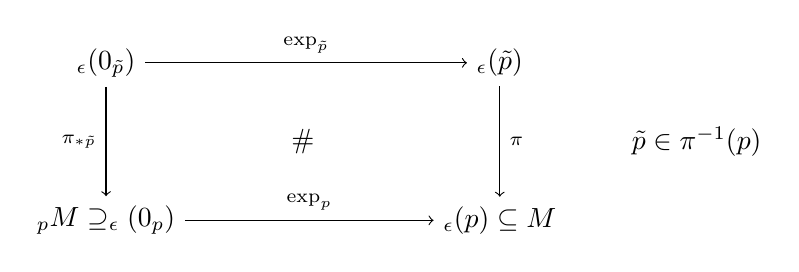
\begin{tikzpicture}
	\def\hor{2.5}
	\def\vert{1}
	\node (1) at (-\hor,\vert) {$\B_\epsilon(0_{\tilde p})$};
	\node (2) at (\hor,\vert) {$\B_\epsilon(\tilde p)$};
	\node (3) at (-\hor,-\vert) {$\T_pM \supseteq \B_\epsilon(0_p)$};
	\node (4) at (\hor,-\vert) {$\B_\epsilon(p) \subseteq M$};
	\node at (0,0) {$\#$};
	\node at (2*\hor,0) {$\tilde p \in \pi^{-1}(p)$};
	
	\draw[->] (1) --node[above,font=\scriptsize]{$\exp_{\tilde p}$} (2);
	\draw[->] (3) --node[above,font=\scriptsize]{$\exp_{p}$} (4);
	\draw[->] (1) --node[left,font=\scriptsize]{$\pi_{*\tilde{p}}$} (3);
	\draw[->] (2) --node[right,font=\scriptsize]{$\pi$} (4);
\end{tikzpicture}\end{center}
F"ur hinreichend kleines $\epsilon > 0$ ist $\exp$ ein Diffeomorphismus und das folgende Diagramm kommutiert.
Damit ist $\pi_{\B_\epsilon(\tilde p)}$ ein Diffeomorphismus.
W"aren f"ur $\tilde p_1$ und $\tilde p_2$ die $\epsilon$-B"alle nicht disjunkt und es existiere eine nichttriviale Geod"atische der L"ange $< 2 \epsilon$ von $\tilde p_1$ nach $\tilde p_2$ und damit eine Geod"atische von $p$ nach $p$ der L"ange $< 2 \epsilon$, also in $\B_\epsilon(p)$.
Also sind $\B_\epsilon(\tilde p_1)$ und $\B_\epsilon(\tilde p_2)$ f"ur $\tilde p_1 \ne \tilde p_2$ disjunkt.
\end{bew}

\begin{Prop}
Es seien $\tilde M$ und $M$ zusammenh"angenden Riemannsche Mannigfaltigkeiten und $\pi: \tilde M \to M$ eine Riemannsche "Uberlagerung . Dann ist $\tilde M$ genau dann vollst"andig, wenn $M$ vollst"andig ist.
\end{Prop}

\begin{bew}\begin{description}[font=\normalfont]
\item[\quot{$\Rightarrow$}:]
	Folgt nach Proposition \ref{prop-9-12}
\item[\quot{$\Leftarrow$}:]
	Es sei $M$ vollst"andig und $\tilde p_i$ eine Cauchy-Folge in $\tilde M$.
	Dann ist $p_i = \pi(\tilde p_i)$ auch eine Cauchy-Folge, denn $\pi$ ist 1-Lipschitz, konvergiert also gegen $p \in M$.
	Dann liegen fast alle $p_i$ in einer Umgebung $U$, so dass $\pi_{U_k}: U_k \to U$ eine Isometrie ist.
	Sei $U_k$ so, dass fast alle $\tilde p_i$ in $U_k$ liegen.
	Dann konvergiert $\tilde p_i$ gegen $\tilde p \in U_i$, mit $\tilde p \in \pi^{-1}(p)$.
\end{description}\end{bew}

F"ur jede zusammenh"angende Riemannsche Mannigfaltigkeit $M$ existiert eine bis auf Isometrie eindeutige einfachzusammenh"angende Riemannsche "Uberlagerung $\tilde M$.
Betrachte die topologisch universelle "Uberlagerung $\tilde M$ von $M$.
Zieht man die differenzierbare und geometrische Struktur von $M$ auf $\tilde M$ zurück, so wird $\tilde M$ zu einer Riemannschen Mannigfaltigkeit und die "Uberlagerungsabbildung zu einer Riemannschen "Uberlagerung,

\emph{Problem:} Es ist nicht klar, warum $\tilde M$ eine abz"ahlbare Basis der Topologie hat.
Es gibt dabei zwei Auswege, zum Einen kann man zeigen dass $\pi_1(M)$ abz"ahlbar ist (Diplomarbeit von M. Mermann), die andere M"oglichkeit ist in \quot{Foundations of Differential Geometry}, Band I, Appendix 2 \cite{kobayashi-nomizu1963foundations-diffgeo} beschrieben.

Die Fundamentalgruppe $\pi_1(M)$ ist isomorph zur Gruppe der Decktransformationen:
\begin{center}\begin{tikzpicture}
%	\tikzgitter{(-4,-4)}{(4,4)}
	
	\node at (1.5,1) {$\tilde M$}; \node at (1.5,-1) {$M$};
	
	\coordinate (p) at (-1.5,-1); \coordinate (tildeq) at (-1.5,0.5); \coordinate (tildep) at (-1.5,1.5);
	\fill (p) circle(0.05)node[left,font=\scriptsize]{$p$} (tildeq) circle(0.05)node[left,font=\scriptsize]{$[c](\tilde p)=\tilde q$} (tildep) circle(0.05)node[left,font=\scriptsize]{$\tilde p$};
	
	\draw (p) ..controls(0.5,-3) and (0.5,1)..node[right,font=\scriptsize]{$c$} (p);
	\draw (tildeq) ..controls(0.5,-1) and (0.5,3).. (tildep);
\end{tikzpicture}\end{center}
Jede Decktransformation ist glatt, also ein Diffeomorphismus, und sogar eine Isometrie, da $\pi$ eine lokale Isometrie ist. Jedes Element von $\pi_1(M)$ induziert eine Isometrie von $\tilde M$.

\section{Wirkung diskreter Gruppen}
Es seien $\Gamma$ eine diskrete Gruppe und $X$ eine Menge.
Eine \CmMark{Wirkung} von $\Gamma$ auf $X$, geschrieben $\Gamma \curvearrowright X$, ist ein Gruppenhomomorphismus $\rho: \Gamma \to \Sym(X)$, schreibe $\rho(\gamma)(x) = \gamma.x$, und insbesondere gilt $\gamma(\delta, x) = (\gamma \delta).x$ und $1_\Gamma.x = x$.
Ist $\Gamma \curvearrowright$ eine Wirkung, so bezeichnet $\Gamma.x = \{\gamma.x | \gamma \in \Gamma\}$ die \CmMark{Bahn} oder den \CmMark{Orbit} von $x$ und $\Gamma_x = \{\gamma \in \Gamma | \gamma.x = x \}$ die \CmMark{Isotropieuntergruppe} von $\Gamma$ in $x$.
Jede Wirkung induziert eine "Aquivalenzklassenrelation auf $X$:
\begin{align*}
	x \sim y \Leftrightarrow \exists \gamma \in \Gamma: \gamma.x = y \Leftrightarrow y \in \Gamma.x
\end{align*}
Die "Aquivalenzklasse $[x]_\sim$ ist also genau die Bahn durch $x$.
Der Quotient $\FakRaum{X}{\Gamma} = \FakRaum{x}{\sim} = \bigcup \Gamma.x$ hei"st \CmMark{Bahnenraum} der Wirkung , die Abbildung $X \to \FakRaum{X}{\Gamma}, x \mapsto [x]_\sim$ die \CmMark[Projektion!kanoniche]{kanonische Projektion}.
Eine Wirkung hei"st \CmMark[Wirkung!freie]{frei}, wenn f"ur alle $x \in X$ $\Gamma_x = \{ 1_\Gamma \}$ gilt.
Es sei $M$ eine Riemannsche Mannigfaltigkeit und $\Gamma$ eine glatte oder isometrische Wirkung, das hei"st $\rho: \Gamma \to \Diff(M)$ oder $\rho: \Gamma \to \Iso(M)$.
Eine solche Wirkung hei"st \CmMark[Wirkung!eigentlich diskontinuierliche]{eigentlich diskontinuierlich}, wenn f"ur jedes Kompaktum $K \subseteq M$ mit $\# \{ \gamma \in \Gamma | \gamma.K \cap K \ne \emptyset \} < \infty$; in diesem Fall ist $\FakRaum{\Gamma}{\Gamma}$ Hausdorffsch.
Ist diese Wirkung zudem frei, so ist der Bahnenraum $\FakRaum{\Gamma}{\Gamma}$ in nat"urlicher Weise eine (Riemannsche) Mannigfaltigkeit und die kanonische Projektion $\pi: M \to \FakRaum{M}{\Gamma}$ eine Riemannsche "Uberlagerung.

\begin{Bsp}\begin{enumerate}[label=\arabic*),leftmargin=*]
\item
	Ist $\pi: \tilde M \to M$ eine universelle Riemannsche "Uberlagerung, so ist $\pi_1(M) \curvearrowright \tilde M$ frei und eigentlich diskontinuierlich und isometrisch, der Quotient $\FakRaum{\tilde M}{\pi_1(M)}$ ist isometrisch zu $M$.
\item
	Betrachte die Wirkung $\Z^2 \curvearrowright \R^2$ durch Translationen $(a,b).(x,y) = (x+a, y+b)$. Die Wirkung von $\Z^2$ auf $\R^2$ ist isometrisch, frei und eigentlich diskontinuierlich.
	\begin{bew}
	Der Quotient $\FakRaum{\R^2}{\Z^2}$ ist diffeomorph zum Torus $T^2 = S^1 \X S^1$.
	Die glatte Abbildung $\R^2 \to T^2$, $(x,y) \mapsto (e^{2 \pi i x}, e^{2 \pi i x})$ faktorisiert "uber die Wirkung und induziert einen Diffeomorphismus.
	\begin{center}\begin{tikzpicture}[font=\scriptsize]
%		\tikzgitter{(-5,-5)}{(5,5)}
		
		\def\step{0.75}
		
		%\filldraw[pattern=north east lines] (0,0) rectangle (\step,\step);
		\fill[fill=gray!20] (0,0) rectangle (\step,\step);
		\draw (-\step,0) -- (6*\step,0) (0,-\step) --node[left,pos=0.6]{$\R^2$} (0,5*\step);
		\foreach \i in {0,1,...,5}{
			\foreach \j in {0,1,...,4}{
				\fill (\i*\step,\j*\step) circle(0.05);
			}
		}
		\fill (4.5*\step,3.5*\step)node[right]{$x$} circle(0.05);
		\fill (0.5*\step,0.5*\step) circle(0.05) (0.3*\step,\step) circle(0.05) node[above]{$y$} (0.3*\step,0) circle(0.05) node[below]{$y'$};
		
		\coordinate(sqr) at (-0.5,-2);
		\def\seite{0.75}
		% neuer Befehl fuer einen kurzen schraegen strich
		\filldraw[fill=gray!20] ($(sqr)-(\seite,\seite)$) rectangle ($(sqr)+(\seite,\seite)$);
		\newcommand{\strich}[1]{
			\def\hor{0.05}
			\def\vert{0.1}
			\draw ($#1 - (\hor,\vert)$) -- ($#1 + (\hor,\vert)$);
		}
		\strich{($(sqr)+(0,\seite)$)}
		\strich{($(sqr)+(0,-\seite)$)}
		% doppelt gestrichen, zwei vertikal versetzte Striche
		\newcommand{\sstrich}[1]{
			\strich{($#1-(0,0.05)$)}
			\strich{($#1+(0,0.05)$)}
		}
		\sstrich{($(sqr)-(\seite,0)$)}
		\sstrich{($(sqr)+(\seite,0)$)}
		
		\coordinate (tor) at (4.75,-2);
		\tikztorus[0.75]{(tor)}
		
		\draw[gray,dashed,name path=a] (tor) ellipse[x radius=1.2,y radius=0.5];
		\draw[gray,dashed,name path=b] ($0.5*(torusUntenLoch) + 0.5*(torusUnten)$) ellipse[x radius=0.15,y radius=0.28];
		\strich{($(tor) + (0,0.5)$)}
		\path[name intersections={of=a and b}];
		\sstrich{(intersection-1)}
		
		\draw[->] (0.75,-2) ..controls(1.5,-1.75) and (2,-2.25)..node[above]{verkleben} (2.75,-2);
		
		\draw (0.75,-2.5) -- (2.75,-2.5); \draw (0.75,-3) -- (2.75,-3);
		\draw (0.75,-2.75) ellipse[x radius=0.125,y radius=0.25] (2.75,-2.75) ellipse[x radius=0.125,y radius=0.25];
		\draw[gray,dashed] (0.875,-2.75) --coordinate(pkt) (2.875,-2.75);
		\strich{(pkt)}
		\sstrich{(0.625,-2.75)}
		\sstrich{(2.625,-2.75)}
	\end{tikzpicture}\end{center}
	Die durch die Wirkung auf $T^2$ induzierte Metrik ist flach, in dem Sinne dass die Kr"ummung konstant Null ist.
	Die Geod"atischen des  flachen Torus sind genau die Bilder von Geod"atischen des $\R^2$, also von Geraden, unter der kanonischen Projektion.
	\begin{center}\begin{tikzpicture}[font=\scriptsize]
		%\tikzgitter{(-4,-5)}{(8,5)}
		\def\step{0.75}
		
		\fill[fill=gray!20] (0,0) rectangle (\step,\step);
		\draw (-\step,0) -- (6*\step,0) (0,-\step) --node[left,pos=0.6]{$\R^2$} (0,5*\step);
		\foreach \i in {0,1,...,5}{
			\foreach \j in {0,1,...,4}{
				\fill (\i*\step,\j*\step) circle(0.05);
			}
		}
		\fill[gray] (0.33*\step,\step) circle(0.05) (0.33*\step,0) circle(0.05);
		
		\coordinate (vec) at (\step,3*\step);
		\draw[->,gray] ($-0.2*(vec)$) --node[left,pos=0.7]{$\tilde c$} ($1.2*(vec)$); \draw[gray] ($1.2*(vec)$) -- ($1.5*(vec)$);
		\draw[gray,dashed] ($-0.2*(vec) + 0.33*(\step,0)$) -- ($1.5*(vec) + 0.33*(\step,0)$);
		\draw[gray,dashed] ($-0.2*(vec) + 0.66*(\step,0)$) -- ($1.5*(vec) + 0.66*(\step,0)$);
		
		\draw[gray,->] (4,1.5) to[out=290,in=70] (4,0.75);
		\draw[gray,->] (4.125,2.25) to[out=290,in=70] node[right]{$(0,-1)^2 \in \Z^2$} (4.125,0.75);
		
		\coordinate(sqr) at (-0.5,-2);
		\def\seite{0.75}
		% neuer Befehl fuer einen kurzen schraegen strich
		\filldraw[fill=gray!20] ($(sqr)-(\seite,\seite)$) rectangle ($(sqr)+(\seite,\seite)$);
		\newcommand{\strich}[1]{
			\def\hor{0.05}
			\def\vert{0.1}
			\draw ($#1 - (\hor,\vert)$) -- ($#1 + (\hor,\vert)$);
		}
		\strich{($(sqr)+(0,\seite)$)}
		\strich{($(sqr)+(0,-\seite)$)}
		% doppelt gestrichen, zwei vertikal versetzte Striche
		\newcommand{\sstrich}[1]{
			\strich{($#1-(0,0.05)$)}
			\strich{($#1+(0,0.05)$)}
		}
		\sstrich{($(sqr)-(\seite,0)$)}
		\sstrich{($(sqr)+(\seite,0)$)}
		
		\foreach \i in {0,1,2}{
			\coordinate (unten) at ($(sqr) - (\seite,\seite) + (\i/3*2*\seite,0)$);
			\coordinate (oben) at ($(unten) + (2/3*\seite,2*\seite)$);
			\fill[gray] (unten) circle(0.05) (oben) circle(0.05);
			\draw[gray] (unten) -- (oben);
		}
		\path[gray] ($(sqr) - (\seite,\seite) + (2/3*\seite,0)$) --node[right]{$c$} ($(sqr) - (\seite,\seite) + (2/3*\seite,0) + (2/3*\seite,2*\seite)$);
		
		\coordinate (tor) at (4.75,-2);
		\tikztorus[0.75]{(tor)}
		
		%\path (tor) ellipse[x radius=1.5,y radius=0.75];
		\coordinate (1) at ($(tor)+(90:1.5 and 0.75)$); % aussen oben
		\coordinate (2) at ($(tor)+(225:1.5 and 0.75)$); % aussen sued-west
		\coordinate (3) at ($(tor)+(300:1.5 and 0.75)$); % aussen sued-ost
		%\path[draw,green] ($(tor) - 0.75*(0,0.5)$) ellipse (0.75 and 0.75*0.75);
		\coordinate (4) at ($(tor) - 0.75*(0,0.5) + (50:0.75 and 0.75*0.75)$); % innen ost
		\coordinate (5) at ($(tor) - 0.75*(0,0.5) + (135:0.75 and 0.75*0.75)$); % innen west
		%\path[draw,green] ($(tor) + 0.75*(0,0.75)$) ellipse (0.75*1.25 and 0.75*1);
		\coordinate (6) at ($(tor) + 0.75*(0,0.75) + (250:0.75*1.25 and 0.75*1)$); % innen sued
		%\draw[red] (1) circle(0.05); \draw[red] (2) circle(0.05); \draw[red] (3) circle(0.05); \draw[red] (4) circle(0.05); \draw[red] (5) circle(0.05); \draw[red] (6) circle(0.05);
		
		\def\angle{180}
		\coordinate (ctrl1l) at (\angle:0.2); \coordinate (ctrl1r) at (180+\angle:0.2);
		\def\angle{150}
		\coordinate (ctrl2l) at (\angle:0.25); \coordinate (ctrl2r) at (180+\angle:0.25);
		\def\angle{200}
		\coordinate (ctrl3l) at (\angle:0.6); \coordinate (ctrl3r) at (180+\angle:0.3);
		\def\angle{150}
		\coordinate (ctrl4l) at (\angle:0.2); \coordinate (ctrl4r) at (20:0.45);
		\def\angle{210}
		\coordinate (ctrl5l) at (\angle:0.25); \coordinate (ctrl5r) at (180+\angle:0.3);
		\def\angle{160}
		\coordinate (ctrl6l) at (\angle:0.4); \coordinate (ctrl6r) at (180+\angle:0.3);
		
		\draw[gray] (3) ..controls($(3) + (ctrl3r)$) and ($(4) + (ctrl4r)$).. (4) (1) ..controls($(1) + (ctrl1l)$) and ($(5) + (ctrl5r)$).. (5) (2) ..controls($(2) + (ctrl2r)$) and ($(6) + (ctrl6l)$).. (6);
		\draw[dashed,gray] (3) ..controls($(3) + (ctrl3l)$) and ($(6) + (ctrl6r)$)..coordinate[pos=0.6](pkt) node[right,gray]{$c$} (6) (1) ..controls($(1) + (ctrl1r)$) and ($(4) + (ctrl4l)$).. (4) (2) ..controls($(2) + (ctrl2l)$) and ($(5) + (ctrl5l)$).. (5);
		\fill[gray] (pkt) circle(0.05);
		
		\draw[->] (0.75,-2) ..controls(1.5,-1.75) and (2,-2.25).. (2.75,-2);
		
		\node[gray] at (6.5,-3) {$c = \pi \circ \tilde c$};
		\end{tikzpicture}\end{center}	
	\end{bew}
\item
	Der $n$-dimensionale reell-projektive Raum $\R\P^n$: betrachte $\Z_2 \curvearrowright S^n$, $\gamma.p = -p$, $\gamma \ne 1_{\Z_2}$
	\begin{center}\begin{tikzpicture}[font=\scriptsize]
		%\tikzgitter{(-3,-2)}{(3,2)}
		\draw (0,0) circle(1.5);
		\begin{scope}
			\clip (-1.5,0) rectangle (1.5,0.75);
			\draw[dashed] (0,0) ellipse[x radius=1.5, y radius=0.5];
		\end{scope}\begin{scope}
			\clip (-1.5,0) rectangle (1.5,-0.75);
			\draw (0,0) ellipse[x radius=1.5, y radius=0.5];
		\end{scope}
		
		\draw (0,1.5) to[out=310,in=50] (0,-1.5);
		\coordinate (vec) at (0.5,0.5);
		\def\factor{1.5}
		\fill (0,0) circle(0.05);
		\draw[dashed] ($-\factor*(vec)$) node[below right]{$-p$} -- ($\factor*(vec)$) node[right]{$p$};
		\fill ($-\factor*(vec)$) circle(0.05) ($\factor*(vec)$) circle(0.05);
		
		\node at (-2,1.25) {$S^n \curvearrowleft \Z_2$};
		\node[align=left] at (3.5,0) {Geod"atisch minimieren\\bis zur L"ange $\le \frac{\pi}{2}$};
	\end{tikzpicture}\end{center}
	$\R\P^n = \FakRaum{S}{\Z_2}$
	\begin{center}\begin{tikzpicture}[font=\scriptsize]
		%\tikzgitter{(-3,-2)}{(3,2)}
		\begin{scope}
			\clip (-1.75,0) rectangle (1.75,1.75);
			\draw (0,0) circle(1.5);
		\end{scope}\begin{scope}
			\clip (-1.75,0) rectangle (1.75,0.75);
			\draw[dashed] (0,0) ellipse[x radius=1.5, y radius=0.5];
		\end{scope}\begin{scope}
			\clip (-1.75,0) rectangle (1.75,-0.75);
			\draw (0,0) ellipse[x radius=1.5, y radius=0.5];
		\end{scope}
		
		\coordinate (x) at (110:1.5 and 0.5); \coordinate (x') at (290:1.5 and 0.5);
		\fill (x) circle(0.05) node[above left]{$-x$} (x') circle(0.05) node[below right]{$x$};
		
		\coordinate (0) at (330:1.5 and 0.5);
		\node (1) at (3.5,-0.75) {$\FakRaum{S^{n-1}}{\Z_2} = \R\P^{n-1}$};
		\draw[->] (1) to[out=180,in=300] (0);
		\node (2) at (3.5,0.75) {$\R\P^{n}$};
		\draw[right hook->] (1) -- (2);
		\draw[right hook->] ($(2)-(2,0)$) -- (2);
	\end{tikzpicture}\end{center}
\end{enumerate}\end{Bsp}

Es sei $(M, g)$ vollst"andig und $\ric_{(M,g)} \ge (n-1) \frac{1}{r^2} g$ f"ur ein $r > 0$.
Dann erf"ullt auch $\tilde M$ diese Voraussetzungen; insbesondere ist $\tilde M$ (ebenfalls) kompakt. Da $\pi_1(M) \curvearrowright \tilde M$ eigentlich diskontinuierlich wirkt, gilt
\begin{align*}
\# \pi(M) = \# \{ \gamma \in \pi_1(M) | \gamma.\tilde{M} \cap \tilde M \ne \emptyset \} < \infty
\end{align*}

\begin{kor}[zum Satz von Bonnet-Myers]
Unter den Voraussetzungen des Satzes hat $M$ eine endliche Fundamentalgruppe.
\end{kor}

\begin{Satz}[Hadamard-Cartan]
Es sei $(M,g)$ eine vollst"andige Riemannsche Mannigfaltigkeit mit $\sec_{(M,g)} \le 0$. Dann ist f"ur alle $p \in M$ die Exponentialabbildung $\exp_p: \T_pM \to M$ eine "Uberlagerung.
Insbesondere ist jede einfach zusammenh"angende vollst"andige Riemannsche Mannigfaltigkeit mit $\sec \le 0$ diffeomorph zu $\R^m$.
\end{Satz}

\begin{bew}
Es sei $c$ eine Geod"atische und $Y$ ein Jacobifeld entlang $c$ mit $Y(0) = 0$. Dann gilt f"ur $f(t) = \|Y(t)\|^2$:
\begin{align*}
	f'(0) = 2 \langle Y'(0), Y(0) \rangle = 0
\end{align*}
und
\begin{align*}
	f'' &= 2 (\langle Y'', Y \rangle + \langle Y', Y' \rangle)\\
	&= 2 (\|Y'\|^2 - \langle \underbrace{R(Y, \dot c) \dot c, Y}_{=\lambda\sec(\dot c, Y) \le 0}) \ge 0
\end{align*}
Also ist $f$ nichtnegativ und konvex. W"are $Y$ ein nichttriviales Jacobifeld, welches in Punkten $0$ und $t_0$ verschwindet, so folgte aus $f(0) = 0$ und $f(t_0) = 0$, dass $f$, und damit $Y$ verschwindet.
Somit existieren auf $M$ keine zueinander konjugierten Punkte.
Die Exponentialabbildung ist also ein lokaler Diffeomorphismus.
Die Metrik $\tilde g = \exp_{p*}(g)$ auf $\T_pM$ ist nach dem Gau"s-Lemma und dem Satz von Hopf-Rinow vollst"andig.
Nach Proposition \ref{prop-9-12} ist damit $\exp_p(\T_pM, \tilde g) \to (M,g)$ eine Riemannsche "Uberlagerung.
\end{bew}

\begin{emptythm}[Erinnerung (Blatt 12, Aufgabe 2)]
Seien $\gamma_1$ und $\gamma_2$ Geod"atische mit $\gamma_i(0) = p$, $v = \dot\gamma_1(0)$, $w = \dot\gamma_2(0)$ und $\calL(t) = \dop(\gamma_1(t), \gamma_2(t))$. Dann gilt:
\begin{align*}
	\calL(t) = t \|v-w\| \left(1 - \frac{1}{12} \sec(v,w) (1 + \langle v, w \rangle) t^2\right) + o(t^3)\\
	\left(1 - \frac{1}{12} \sec(v,w) (1 + \langle v, w \rangle) t^2\right) + o(t^3) \begin{cases}
		>1 & f"ur \sec < 0\\
		=1 & f"ur \sec = 0\\
		<1 & f"ur \sec > 0
	\end{cases}
\end{align*}
\begin{center}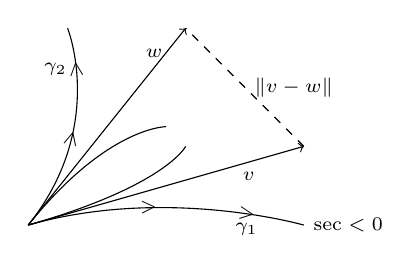
\begin{tikzpicture}[font=\scriptsize]
	%\tikzgitter{(-2,-3)}{(7,3)}
	
	\coordinate (v) at (3.5,1); \coordinate (w) at (2,2.5);
	
	\draw[->] (0,0) --node[below,pos=0.8]{$v$} coordinate[pos=0.5](ctrlv1) (v); \draw[->] (0,0) --node[above,pos=0.8]{$w$} coordinate[pos=0.5](ctrlw1) (w); \draw[dashed] (v) --node[right]{$\|v-w\|$} (w);
	\draw (0,0) ..controls(ctrlw1) and (0.5,2.5).. node[left,pos=0.6]{$\gamma_2$} node[sloped,pos=0.3]{$>$} node[sloped,pos=0.6]{$<$} (0.5,2.5); \draw (0,0) ..controls(ctrlv1) and (3.5,0).. node[below,pos=0.6]{$\gamma_1$} node[sloped,pos=0.3]{$>$} node[sloped,pos=0.6]{$>$} (3.5,0) node[right]{$\sec < 0$};
	\draw (0,0) ..controls(ctrlv1) and (2,1).. (2,1);
	\draw (0,0) ..controls(ctrlw1) and (1.75,1.25).. (1.75,1.25);
\end{tikzpicture}\end{center}
\end{emptythm}

\textbf{Ziel:} Wir suchen ein globales Analogum

\section{Kr"ummungsschranken und Trigonometrie}

\marginnote{\begin{tikzpicture}[font=\scriptsize,scale=0.9]
	%\tikzgitter{(-3,-2)}{(3,2)}
	\tikzsegel{(-2,-1)}
	\coordinate (p) at (-1,-0.75); \coordinate (q) at (0.25,-0.5);
	\fill (p) circle(0.05) node[left]{$p$} (q) circle(0.05) node[above]{$q$};
	\draw (p) to[out=30,in=170] node[above]{$c_v$} (q);
	\draw[->] (-2,1) -- (2,1); \draw[->] (-2,1) -- ++(0.75,1.5);
	\draw[->] (-1,1.25) --node[above,pos=0.8]{$v$} ++(1.25,0.5);
	\fill (-1,1.25) circle(0.05) node[left]{$0_p$};
	\node at (0,-1.75) {$q = \exp_p(v)$};
\end{tikzpicture}}

Es bezeichne $\dop_p$ die Abstandsfunktion $\dop_p(q) = \dop(p, q)$.
Diese ist, in einer punktierten Umgebung von $p$, glatt und es gilt $\dop_p(q) = \| \exp_p^{-1}(q) \|$. Es folgt dann
\begin{align*}
	X(\dop_p)(q) &= \difffrac{}{t} \| \exp_p^{-1}(\exp_p(tX))\|\\
	&= \frac{1}{\| \underbrace{\exp_p^{-1}(q)}_{=v}\|} \langle \exp_{p*v}^{-1}(X), v \rangle\\
	&\overset{\mathclap{\text{G.L.}}}{=} \frac{1}{\|v\|} \langle X, \underbrace{\exp_{p*v}(v)}_{\dot c_v(1)} \rangle \qquad\textcolor{gray}{\text{(nach Gau"s-Lemma)}}
\end{align*}
F"ur eine glatte Funktion $f$ hei"st das durch $X(f) = \langle \grad f, X \rangle$ definierte Vektorfeld der \CmMark{Gradient} von $f$.
Es ist $X(f) = \dop f(X)$ und $\langle \grad f, \cdot \rangle = \dop f$. F"ur den Gradienten von $\dop_p$ gilt nach der obigen Rechnung:
\begin{align*}
	\grad \dop_p = \frac{\exp_{p*v}(v)}{\|v\|} = \frac{\dot c(1)}{\|\dot c(0)\|} = \frac{\dot c(1)}{\|\dot c(1)\|},
\end{align*}
also $\|\grad \dop_p\| \equiv 1$. Eine Funktion $f: U \to \R$, $U$ offen in $M$, hei"st \CmMark[Abstandsfunktion!lokale]{lokale Abstandsfunktion}, wenn $\|\grad f|| \equiv 1$ gilt.
F"ur $p \in U$ sei $c_p$ die Integralkurve von $\grad f$ mit $c_p(f(p)) = p$. Ist $c$ eine (st"uckweise) glatte Kurve von $p$ nach $q$, so gilt
\begin{align*}
	\calL(c) = \int_0^1 ||\dot c\| \overset{C.S.}{\ge} \left| \int_0^1 \langle \grad f, \dot c \rangle \right| = | f(q) - f(p) |
\end{align*}
wobei Gleichheit genau dann gilt, wenn $c$ eine monotone Reparametrisierung von $c_p$ ist. Damit ist $c_p$ eine (minimale) Geod"atische, welche die Niveaumengen von $f$ durchl"auft.
Es gilt
\begin{align*}
	H_f(X, Y) &= X(Y, f) - (\nabla_X Y)(f)\\
	&= X \langle \grad f, Y \rangle - \langle \grad f, \nabla_x Y \rangle\\
	&= \langle \nabla_X \grad f, Y \rangle
\end{align*}
und mit $\|\grad\| \equiv 1$ folgt
\begin{align*}
	0 &= \frac{1}{2} X \|\grad f\|^2\\
	&= \langle \nabla_X \grad f, \grad f \rangle\\
	&= H_f(X, \grad f).
\end{align*}
F"ur ein $r \in \R$ sei $M_r = f^{-1}(r)$ eine Niveaufl"ache von $f$.
Ist $X$ tangential zu $M$, das hei"st existiert eine Integralkurve $\gamma$ von $X$ in $M$, dann gilt
\begin{align*}
	0 = \difffrac[t=0]{}{t} (f(\gamma(t))) = X(f) = \langle \grad f, X \rangle,
\end{align*}
also ist $\grad f$ orthogonal zu $M_r$. F"ur zu $M_r$ tangentiale Vektorfelder $X$ und $Y$ gilt dann
\begin{align*}
	0 = X \langle \grad f, Y \rangle = \langle \nabla_X \grad f, Y \rangle + \langle \grad f, \nabla_X Y \rangle
\end{align*}
also $H_f(X,Y) = - \langle \grad f, \nabla_X Y \rangle$. F"ur $p \in U$ wird durch $X \mapsto \nabla_X \grad f$ ein linearer Endomorphismus $A_p: \grad f^\perp \to \grad f^\perp$ definiert.
Es bezeichne
\begin{align*}
	A_t = A_{c_p(t)}: \underset{\mathclap{\textcolor{gray}{\grad f|_{c_p(t)}}}}{\dot{c}_p(t)^\perp} \to \dot c_p(t)^\perp
\end{align*}
eine Einschr"ankung auf $c_p$. Es sei $\sigma: (-\epsilon, \epsilon) \to M_r$ eine glatte Kurve mit $\sigma(0) = p$.
\begin{center}\begin{tikzpicture}[font=\scriptsize]
	%\tikzgitter{(-7,-4)}	{(7,4)}
	\coordinate (pkt) at (-3,-2);
	\coordinate (p) at (0.75,-0.75);
	\coordinate (0) at ($(p) + (-1.75,-0.25)$);
	\coordinate (1) at ($2*(p) - (0)$);
	\coordinate (ctrlp) at (1,0.5);
	\coordinate (perp) at (-1, 2);
	
	\tikzsegel[2]{(pkt)}
	\tikzsegel[2]{($(pkt) + (-1.25,1.25)$)}
	
	\fill (p) circle(0.05) node[below]{$p$};
	\draw (0) ..controls(0) and ($(p) - (ctrlp)$).. (p) ..controls($(p) + (ctrlp)$) and (1)..node[above,pos=0.7]{$\sigma$} (1);
	
	\foreach \i in {0,0.09,..., 0.3}{
		\path (0) ..controls(0) and ($(p) - (ctrlp)$).. (p) ..controls($(p) + (ctrlp)$) and (1)..coordinate[pos=\i] (pkt) (1);
		\fill (pkt) circle(0.05);
		\draw (pkt) to[bend right=20] coordinate[pos=0.7](k) ++(-2,2);
		\draw[dashed] (pkt) to[bend left=10] ($(pkt) - (-0.25,1)$);
		\fill (k) circle(0.05);
	}
	\path (pkt) circle(0.05) node[below right]{$\sigma(s)$};
	\node at ($(k)+(0.6,0)$) {$\grad f$};
	\node at (-1.5,1) {$c_p$}; \node at (-0.25,1.75) {$c_{\sigma(s)}$};
	
	\begin{scope}
		\clip (p) ..controls($(p) + (ctrlp)$) and (1).. (1) -- ($(p) + (-2,2)$) to[bend left=20] (p) -- (1);
		\draw (p) circle (0.2);
		\fill ($(p) + (60:0.125)$) circle (0.025);
	\end{scope}
	
	\draw[->] (p) -- ++($0.7*(perp)$);
	\draw[->] (2,0.5) -- ++(-0.25,1);\draw[->] (2.5,0.25) -- ++(-0.25,1.5); \draw[->] (3.25,0.5) -- ++(0,2);
	
	\node at (5.5,1) {$M_r$}; \node at (4.25,2.25) {$M_R$};
\end{tikzpicture}\end{center}
Dann ist $(t, s) \mapsto c_{\sigma(s)}(t)$ glatt und f"ur alle $s \in (-\epsilon, \epsilon)$ ist dann $c_{\sigma(s)}$ eine Geod"atische durch $\sigma(s)$; also ist $c_s = c_{\sigma(s)}$ eine geod"atische Variation von $c_0 = c_p$.
Es bezeichne $\calJ$ das zugeh"orige Jacobifeld entlang $c_p$.
%%% Local Variables: 
%%% mode: latex
%%% TeX-master: "../skript-diffgeom"
%%% End: 